\documentclass[12pt,utf8,notheorems,compress]{beamer}

\usepackage[utf8]{inputenc}
\usepackage{default}

\usepackage{lmodern,listings}

% \usetheme{Berlin}
\usetheme{Warsaw}
%\useoutertheme{split}
\usecolortheme{seahorse}
\usepackage{kurier}
%\useinnertheme{rectangles}
\setbeamertemplate{navigation symbols}{}
\setbeamertemplate{footline}{}
\setbeamertemplate{headline}{}

\usepackage[english]{babel}
\usepackage[T1]{fontenc} % Trennung bei Woertern mit Umlauten
\usepackage{amssymb,amsmath,amsthm}
\usepackage{mathtools}
\usepackage{url,tikz}
\usepackage{graphicx}
\usepackage{comment,microtype}
\usepackage{listings}
\usepackage{pst-all}
\usepackage{xypic}

\graphicspath{{img/}}

\setlength\parskip{\medskipamount}
\setlength\parindent{0pt}

\title{Space Ops 101}

\subtitle{An Introduction to Spacecraft Control}

\author{Sven Prüfer}

\institute{German Space Operations Center}

\date{27.12.2018\\[0.5cm]
35c3}

%\titlegraphic{
%\includegraphics[width=6cm]{../images/Uni_Aug_Logo_IFM_RGB.png}
%}

\setlength{\unitlength}{1cm}

\begin{document}

\begin{frame}
 \titlepage
\end{frame}

\begin{frame}
  \frametitle{What we will not talk about ...}
  \begin{figure}[!ht]
    \centering
    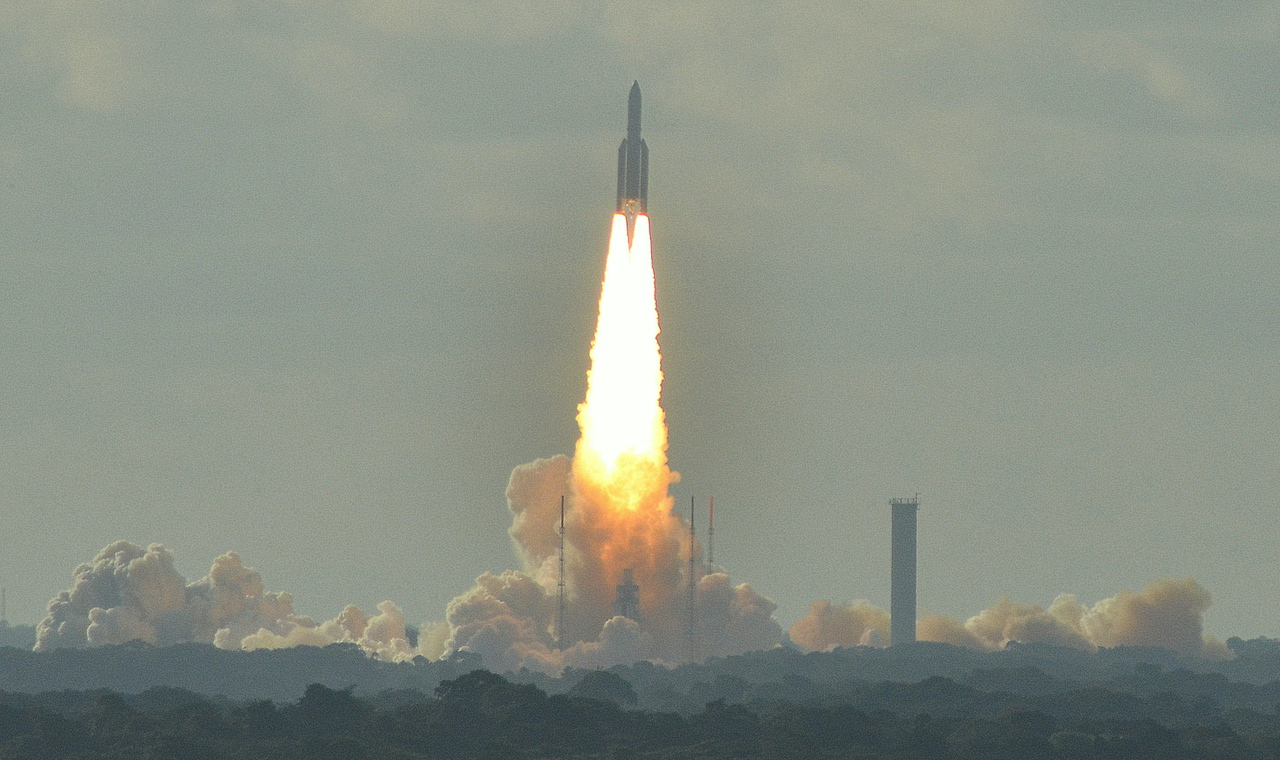
\includegraphics[width=\textwidth]{rocket-launch.jpg}
  \end{figure}
\end{frame}

\begin{frame}
  \frametitle{... but instead}
    \begin{figure}[!ht]
    \centering
    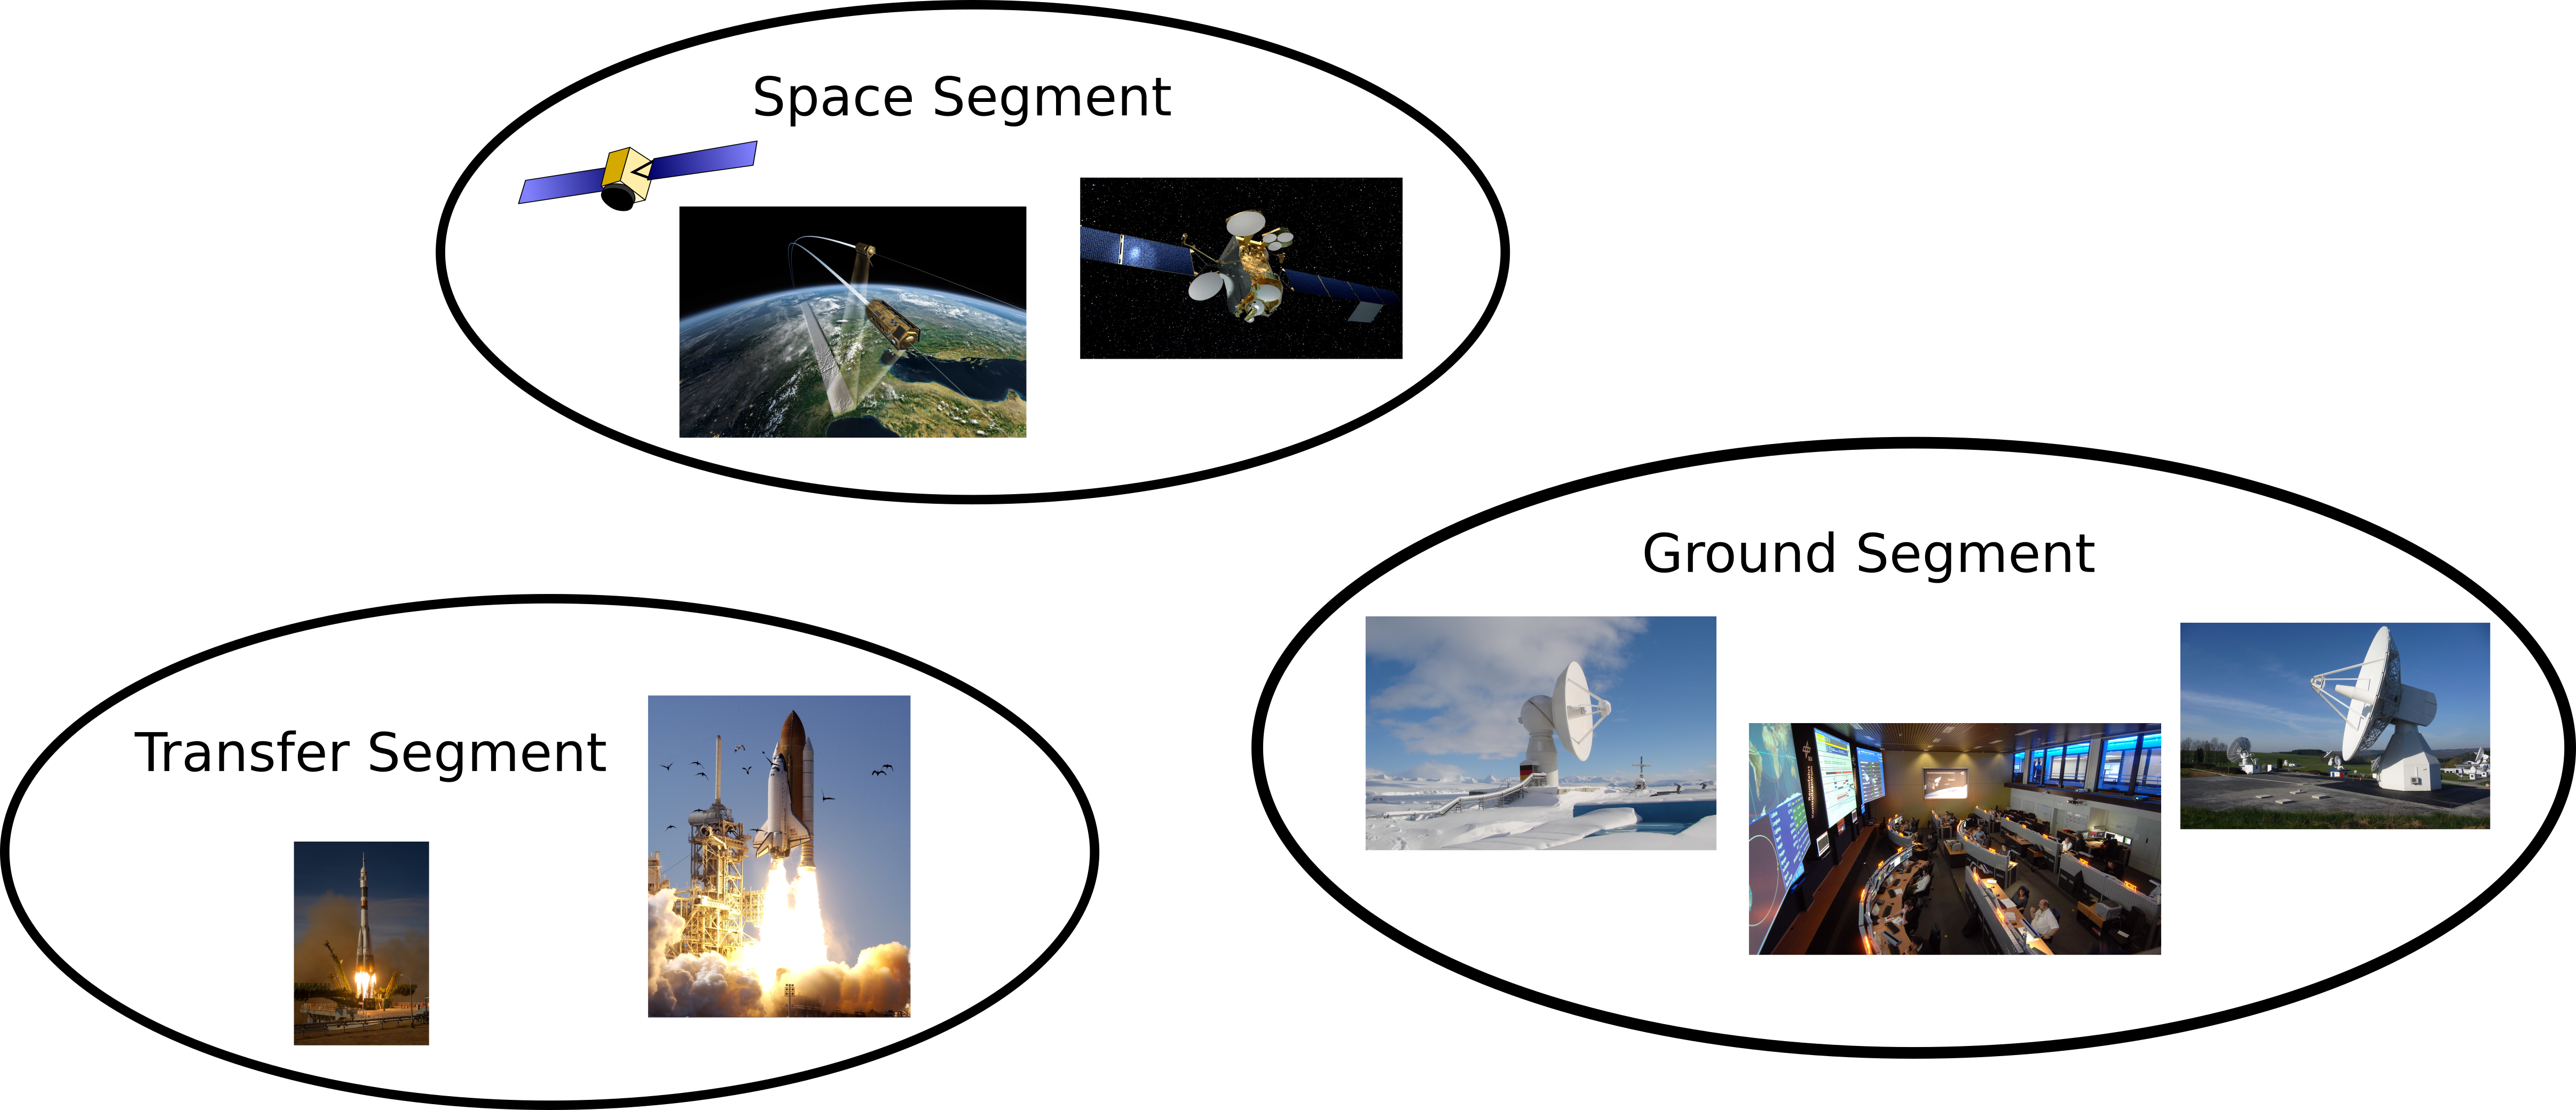
\includegraphics[width=\textwidth]{segments.png}
  \end{figure}
\end{frame}

\begin{frame}
  \frametitle{... but instead}
  \begin{figure}[!ht]
    \centering
    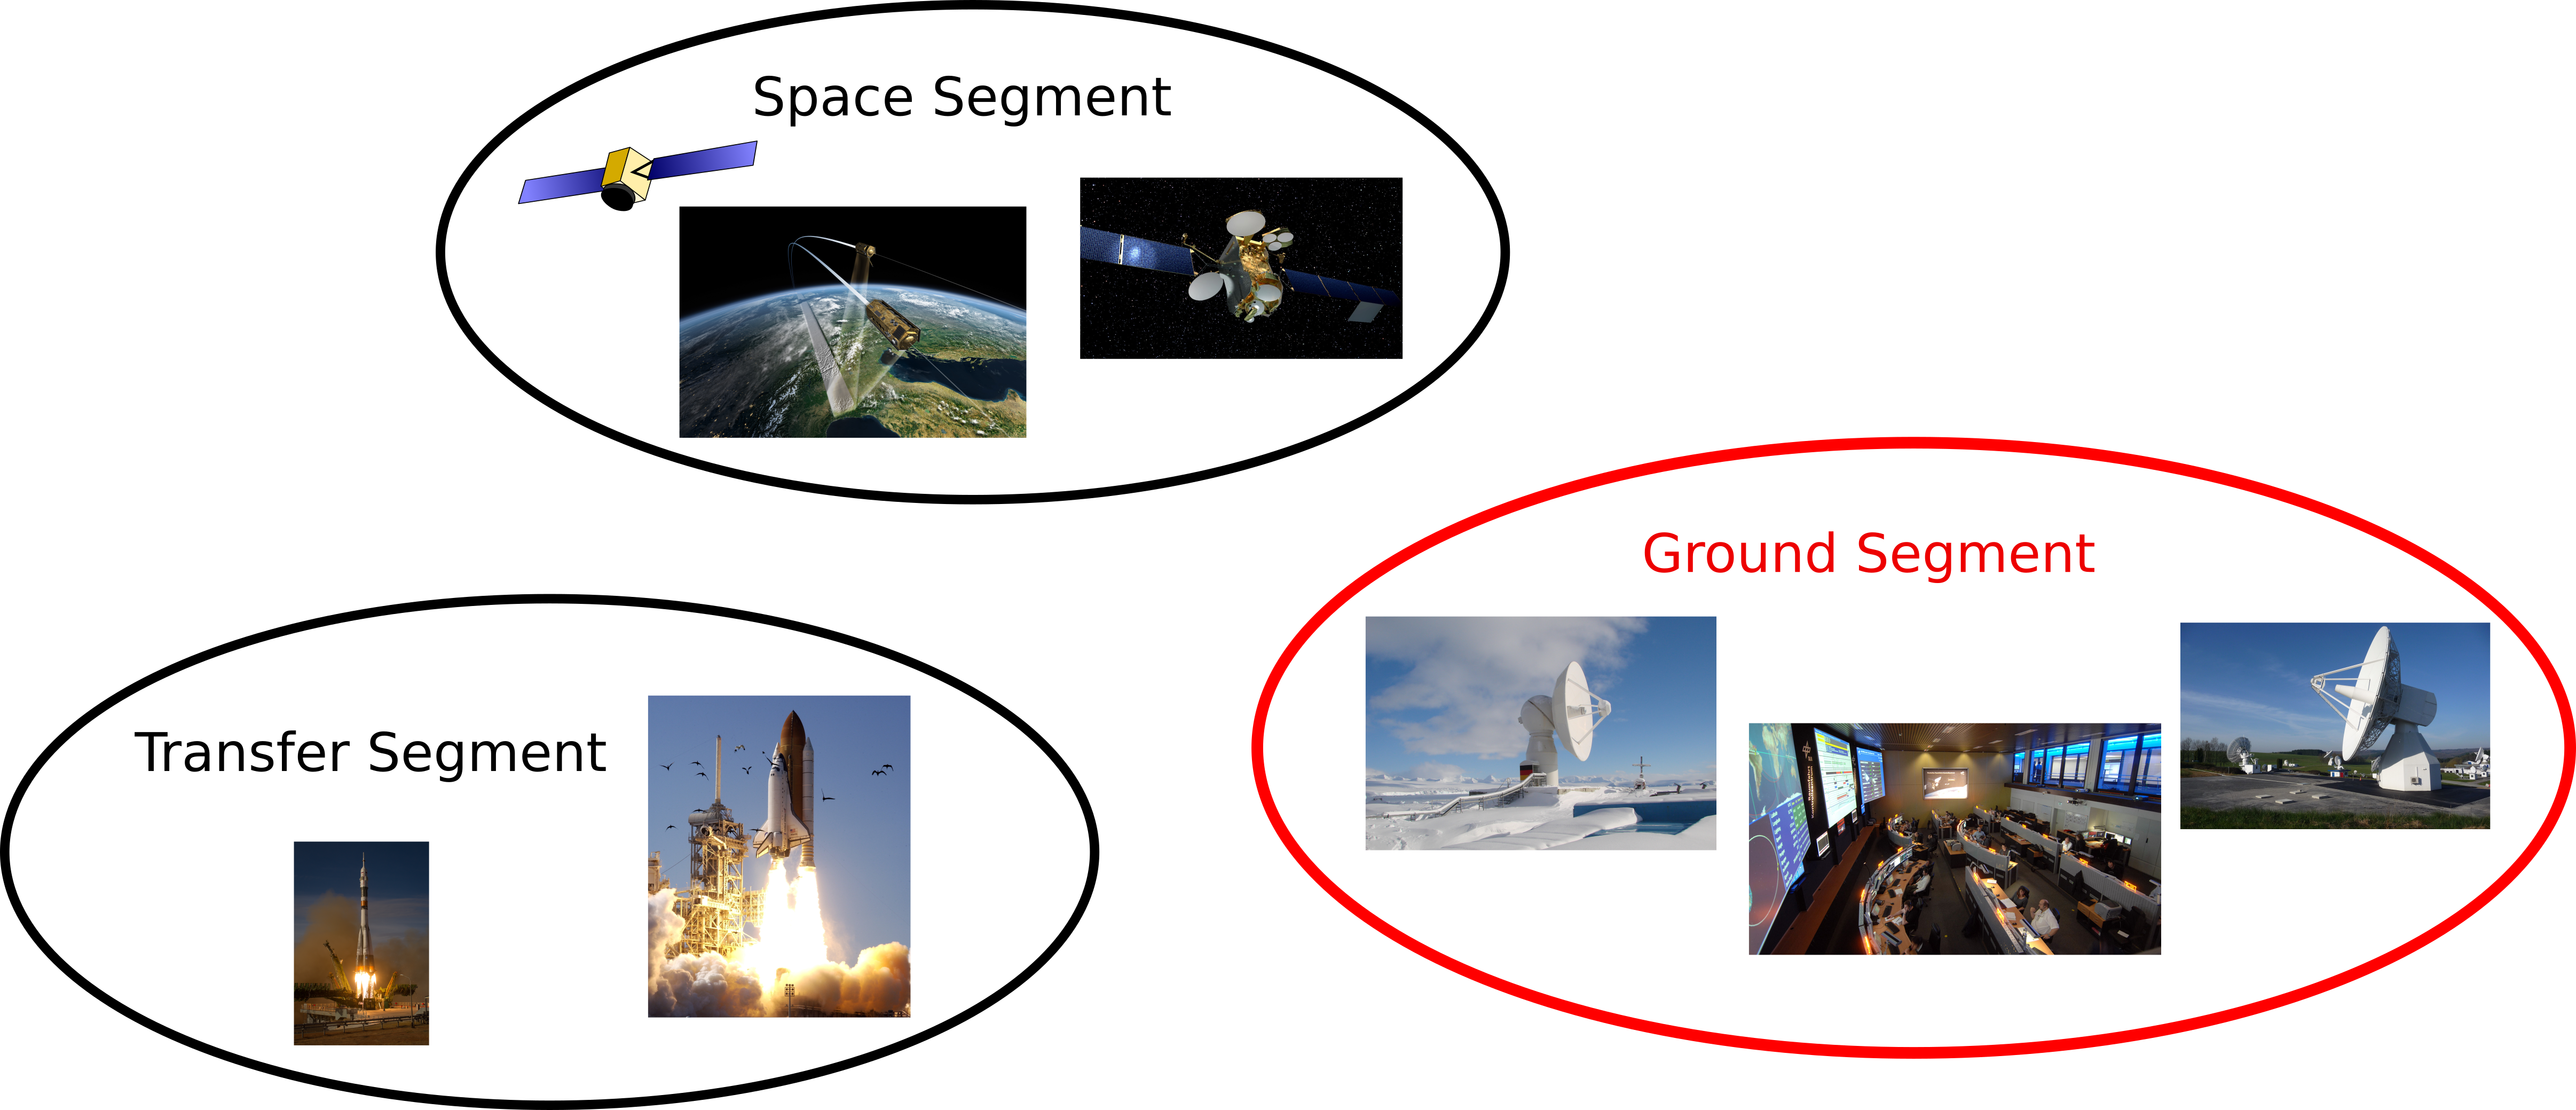
\includegraphics[width=\textwidth]{segments-red.png}
  \end{figure}
\end{frame}

\begin{frame}
  \frametitle{Outline}
  \tableofcontents
\end{frame}

\begin{frame}
  \frametitle{What are we doing here?}
  \pause
  First, a mission needs a name ... such as
  \pause
  \begin{itemize}
    \item \textbf{G}ravity \textbf{R}ecovery \textbf{A}nd \textbf{C}limate \textbf{E}xperiment \pause or
    \item \textbf{Eu}glena and \textbf{C}ombined \textbf{R}egenerative \textbf{O}rganic-Food \textbf{P}roduction \textbf{i}n \textbf{S}pace.
  \end{itemize}
  \pause
  Next, we need a purpose:
  \pause
  \begin{itemize}
    \item Scientific? \pause
    \item Technology Demonstration? \pause
    \item Communications? \pause
    \item TV? \pause
    \item GNSS? \pause
    \item Espionage? \pause
    \item $\ldots$
  \end{itemize}
\end{frame}

\section{Basics of Spaceflight}

\begin{frame}
  \frametitle{}
  \vfill
  \begin{center}
    \Large Basics of Spaceflight
  \end{center}
  \vfill
\end{frame}

\subsection{Orbits}

\begin{frame}
  \frametitle{Why does a space craft not fall down?}
  \pause
  \begin{figure}[b]
    \centering
    
\includegraphics[width=0.8\textwidth]{gravity1.png}
  \end{figure}
\end{frame}

\begin{frame}
  \frametitle{Why does a space craft not fall down?}
  \begin{figure}[b]
    \centering
    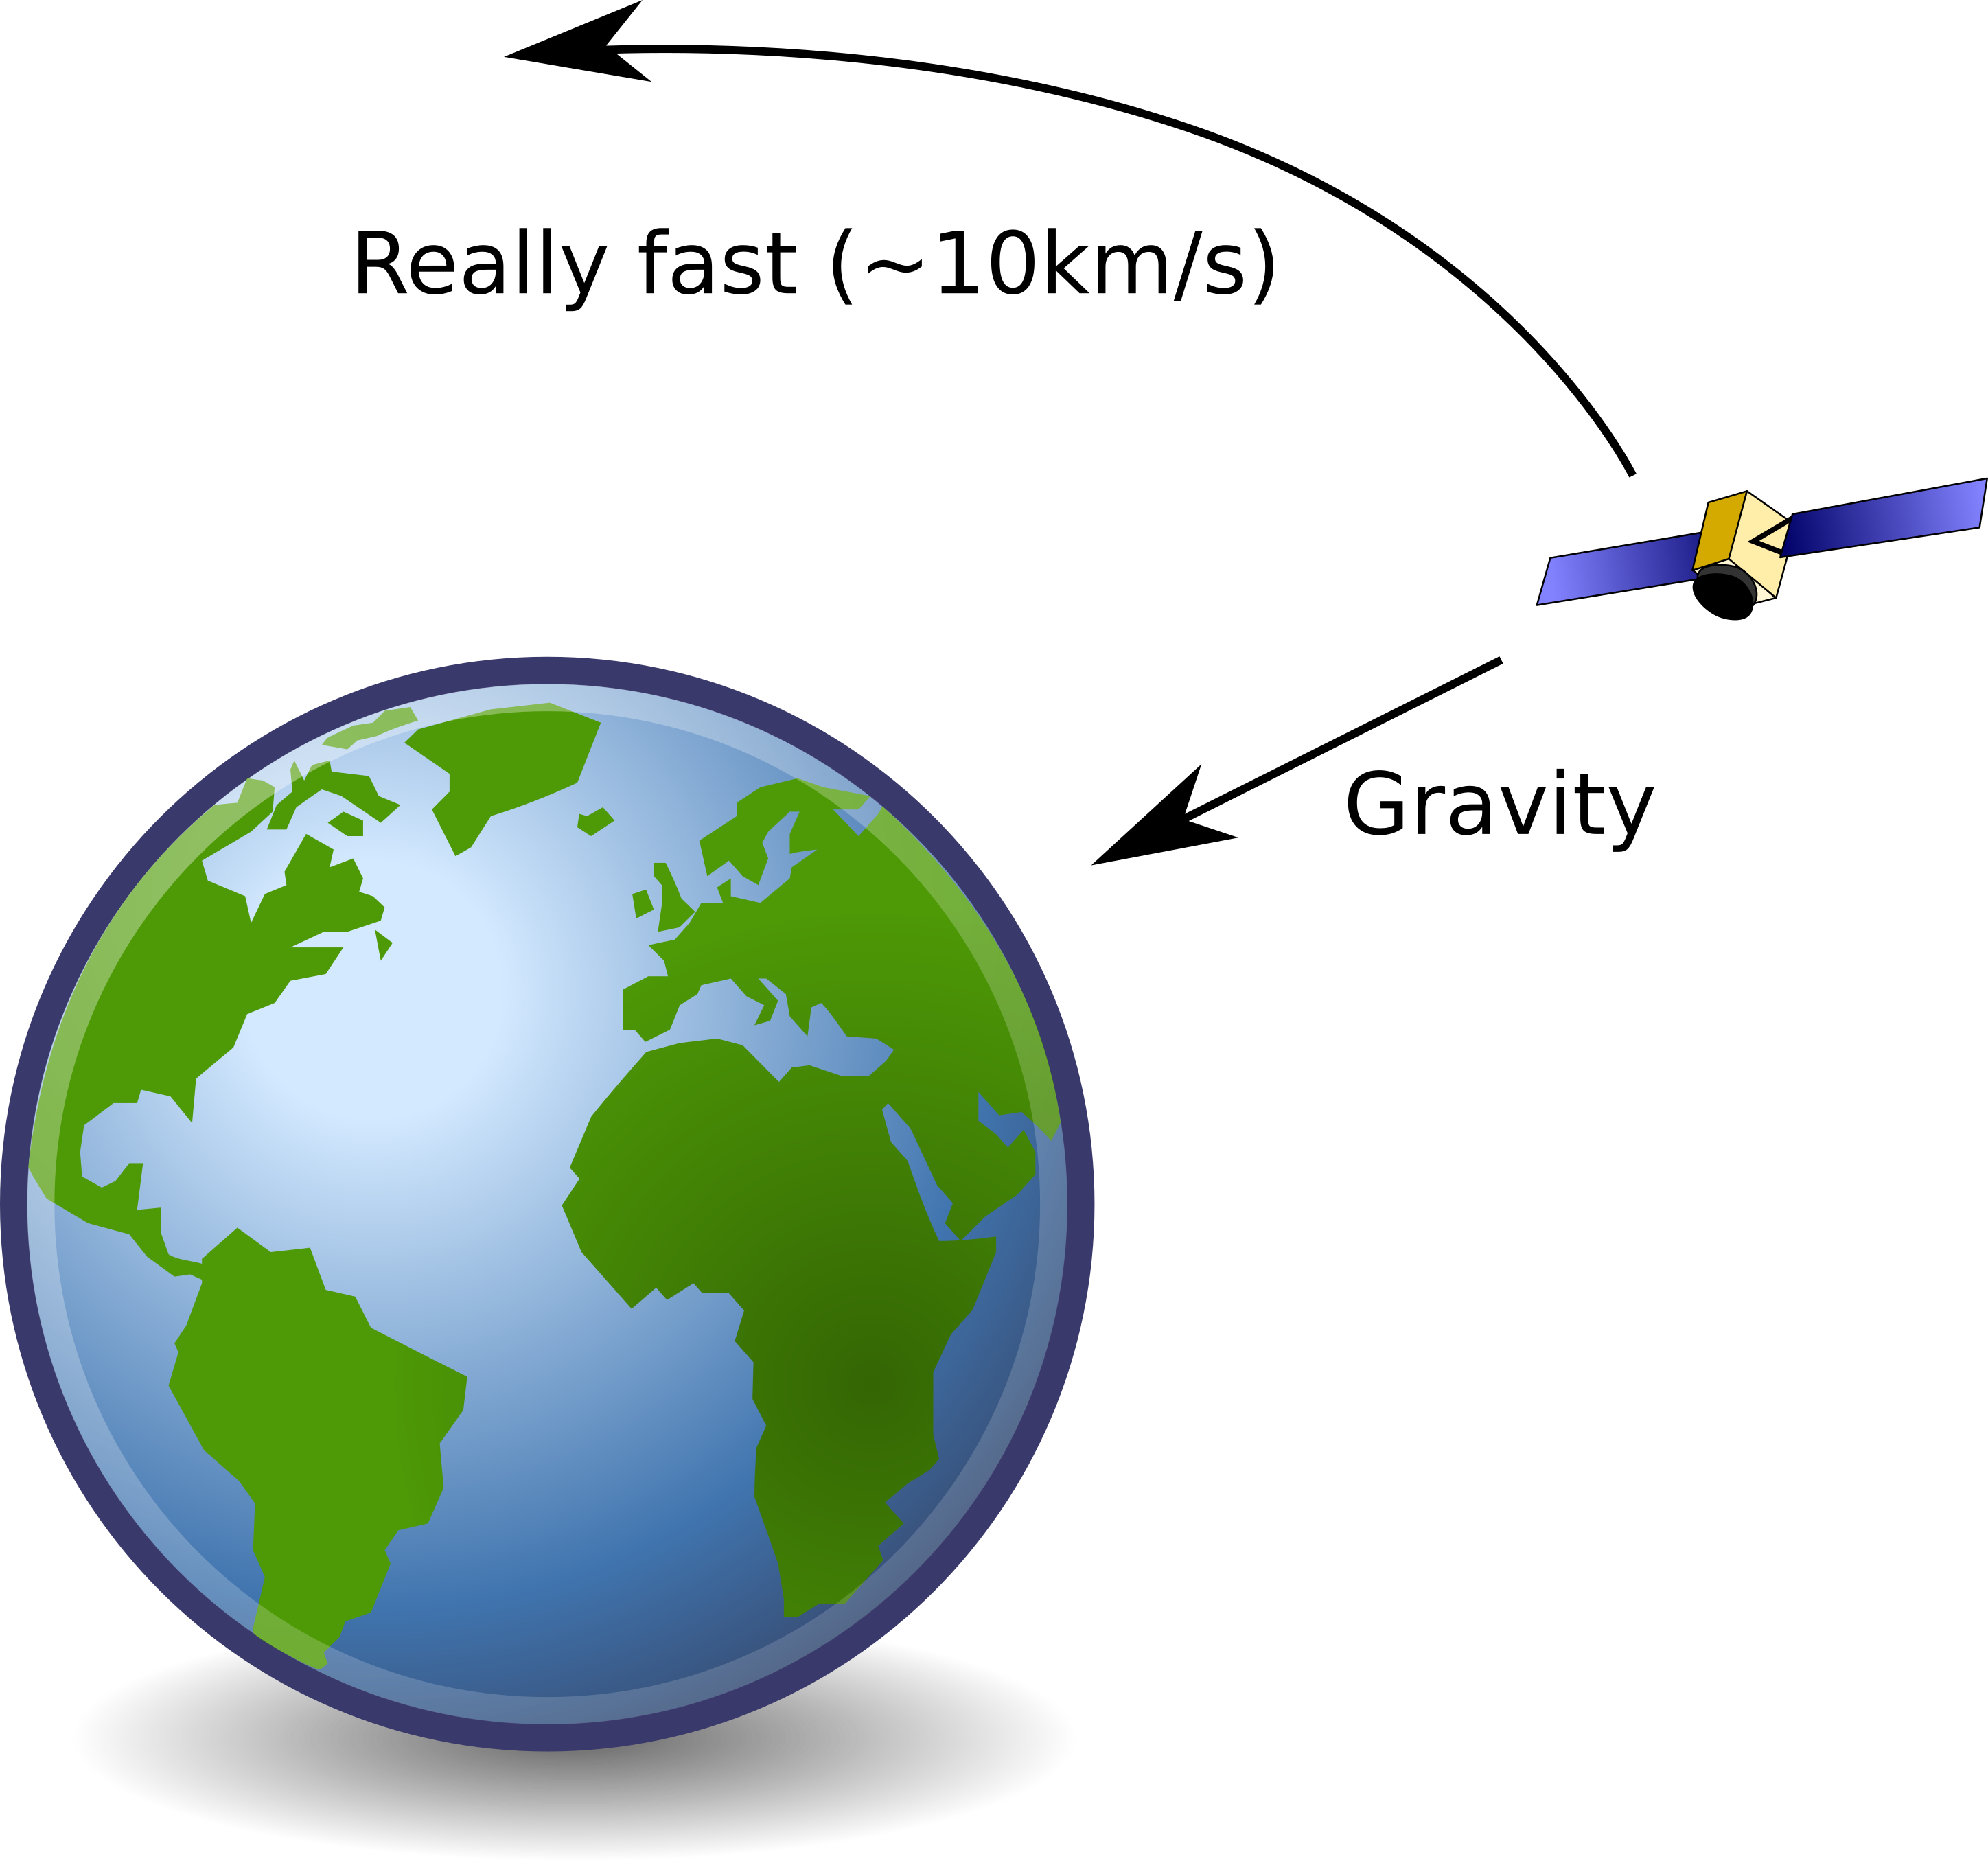
\includegraphics[width=0.8\textwidth]{gravity2.png}
  \end{figure}
\end{frame}

\begin{frame}
  \frametitle{LEO, MEO and GEO}
  \begin{figure}[!ht]
    \centering
    
\includegraphics[width=\textwidth]{orbit1.png}
  \end{figure}
\end{frame}

\begin{frame}
  \frametitle{LEO, MEO and GEO}
  \begin{figure}[!ht]
    \centering
    
\includegraphics[width=\textwidth]{orbit2.png}
  \end{figure}
\end{frame}

\begin{frame}
  \frametitle{LEO, MEO and GEO}
  \begin{figure}[!ht]
    \centering
    
\includegraphics[width=\textwidth]{orbit3.png}
  \end{figure}
\end{frame}

\begin{frame}
  \frametitle{LEO, MEO and GEO}
  \begin{figure}[!ht]
    \centering
    
\includegraphics[width=\textwidth]{orbit4.png}
  \end{figure}
\end{frame}

\subsection{Communications}

\begin{frame}
  \frametitle{Contacts and Passes}
  \pause
  \begin{figure}[!ht]
    \centering
    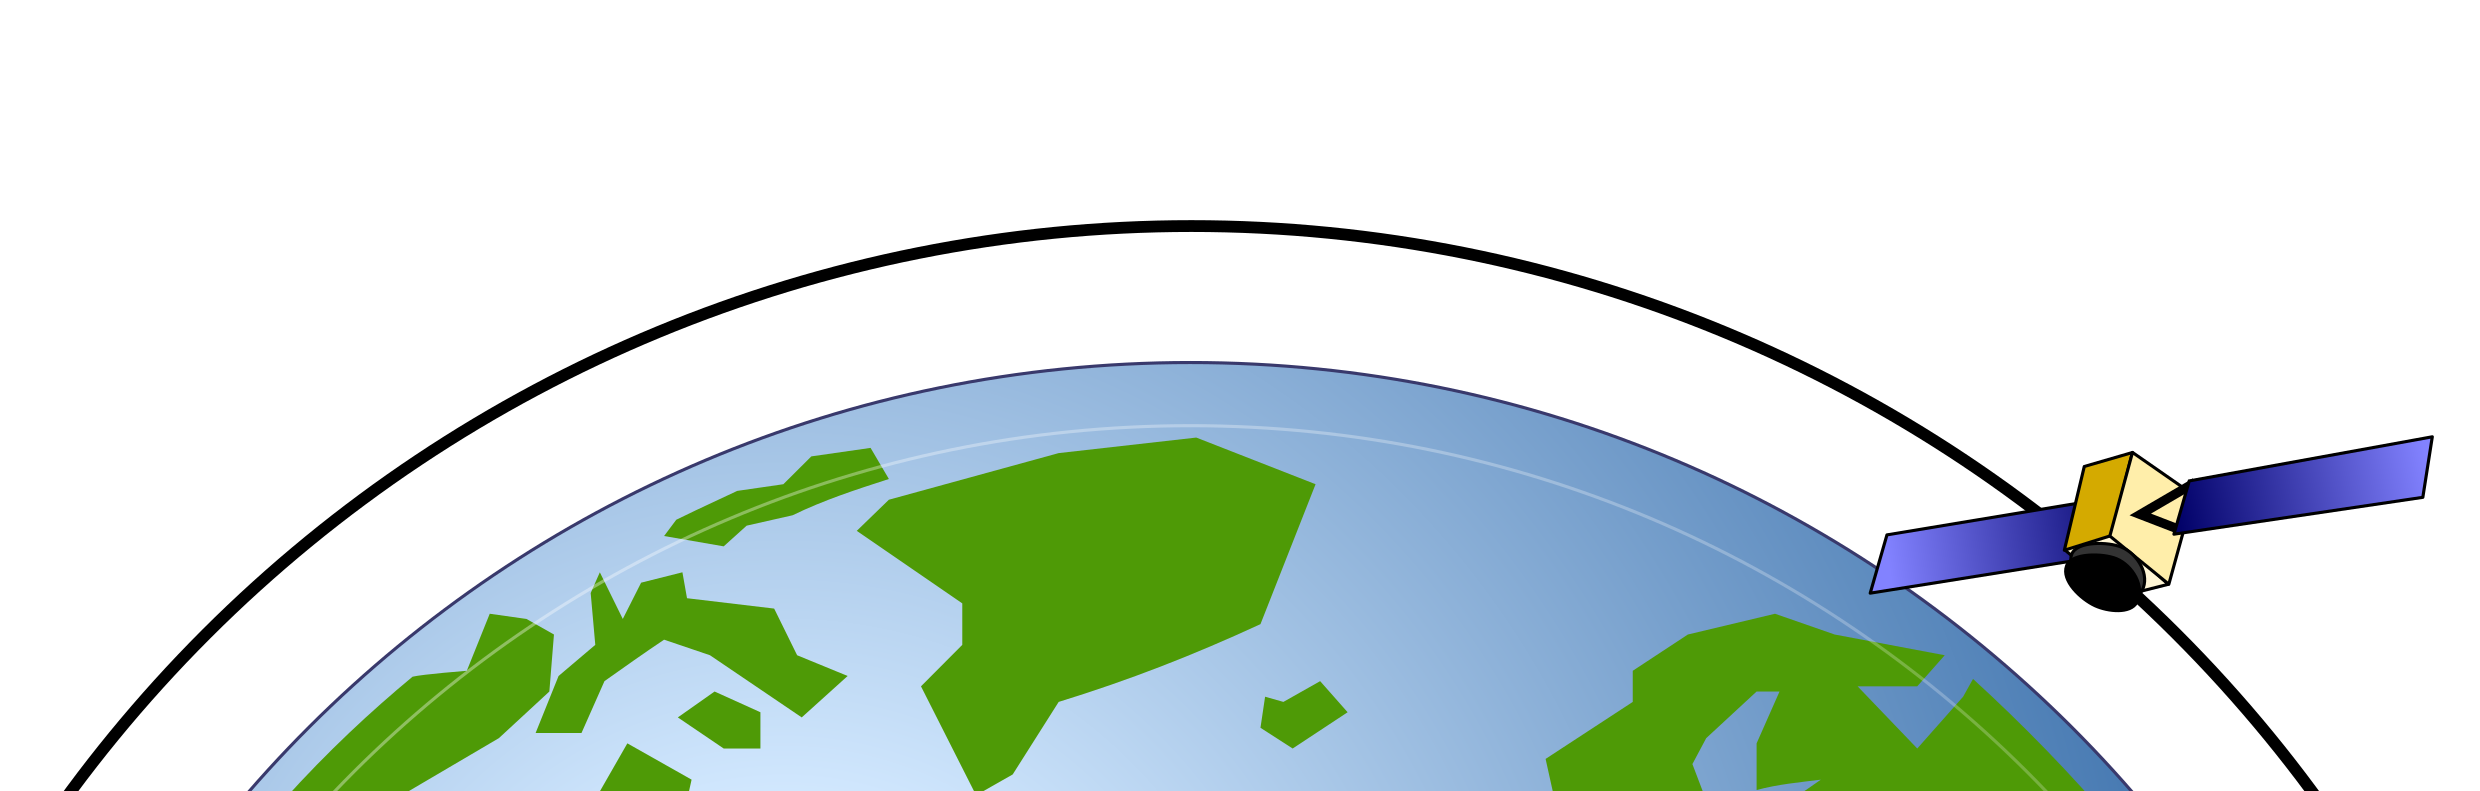
\includegraphics[width=\textwidth]{pass1.png}
  \end{figure}
\end{frame}

\begin{frame}
  \frametitle{Contacts and Passes}
  \begin{figure}[!ht]
    \centering
    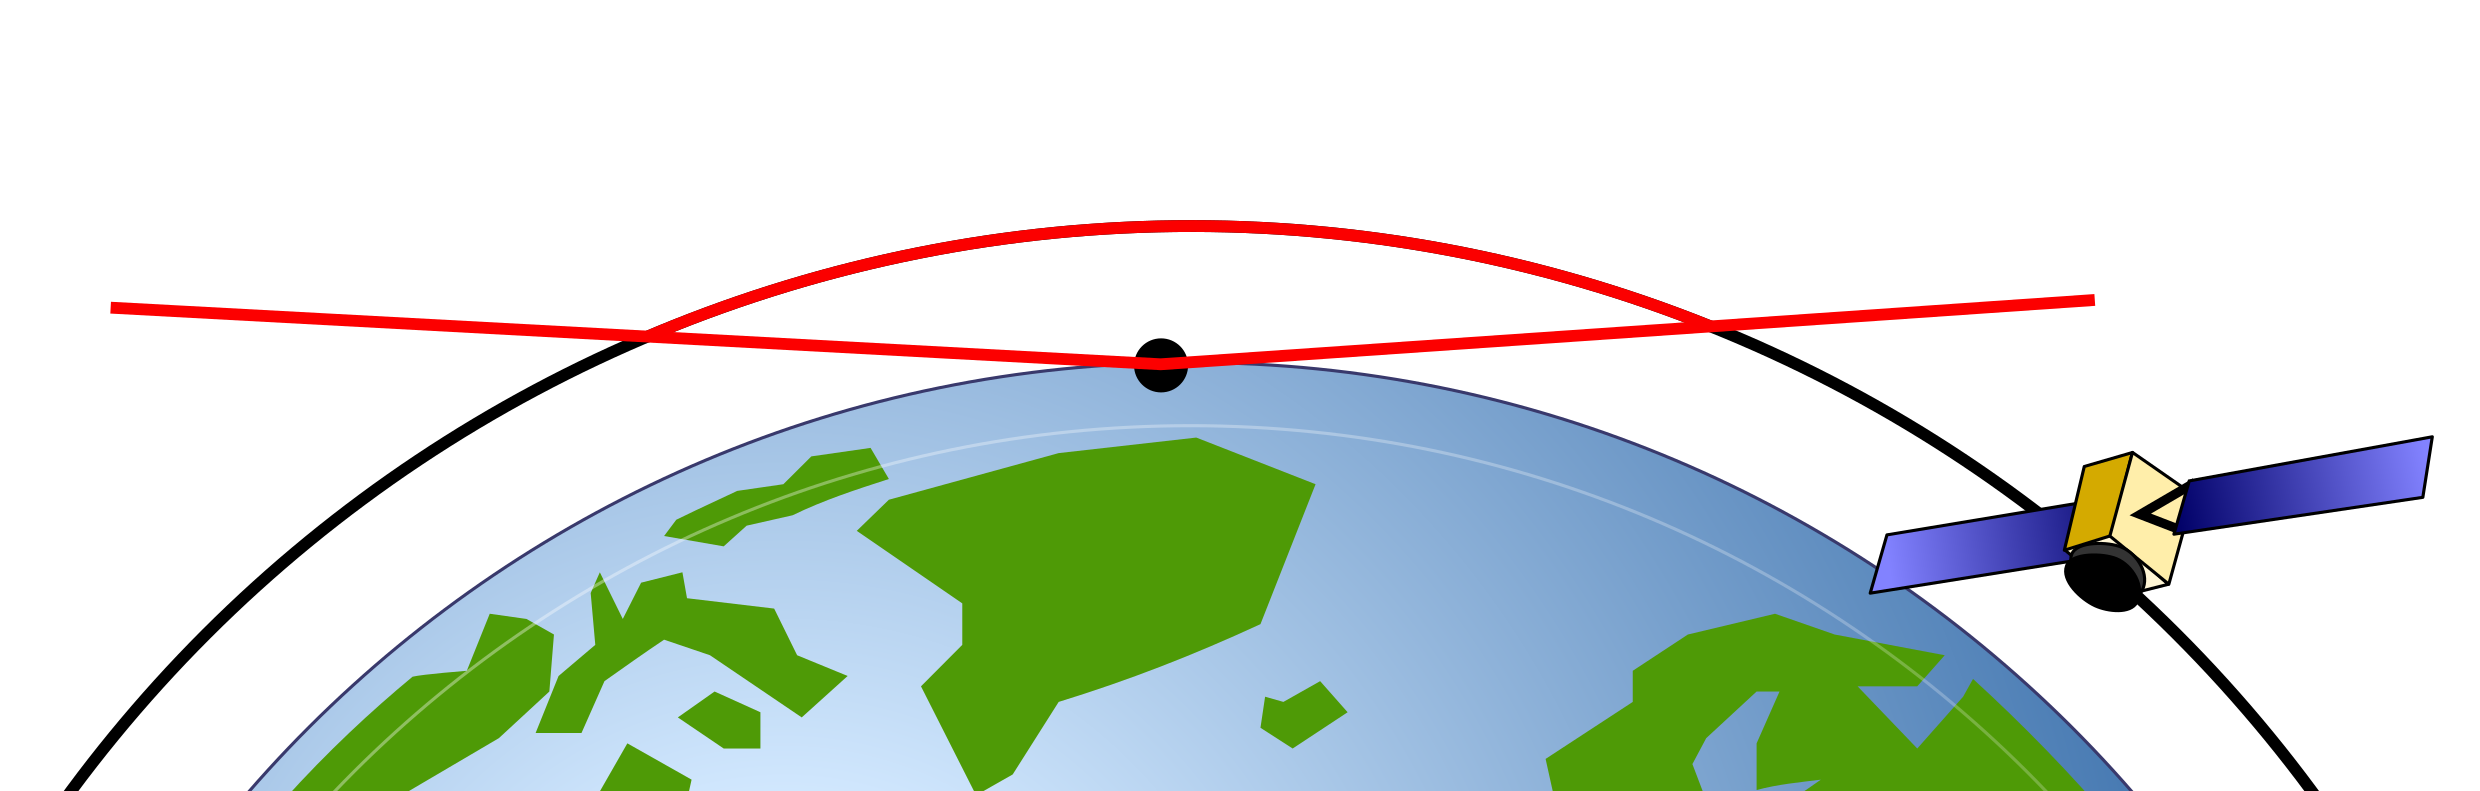
\includegraphics[width=\textwidth]{pass2.png}
  \end{figure}
\end{frame}

\begin{frame}
  \frametitle{Contacts and Passes}
  \begin{figure}[!ht]
    \centering
    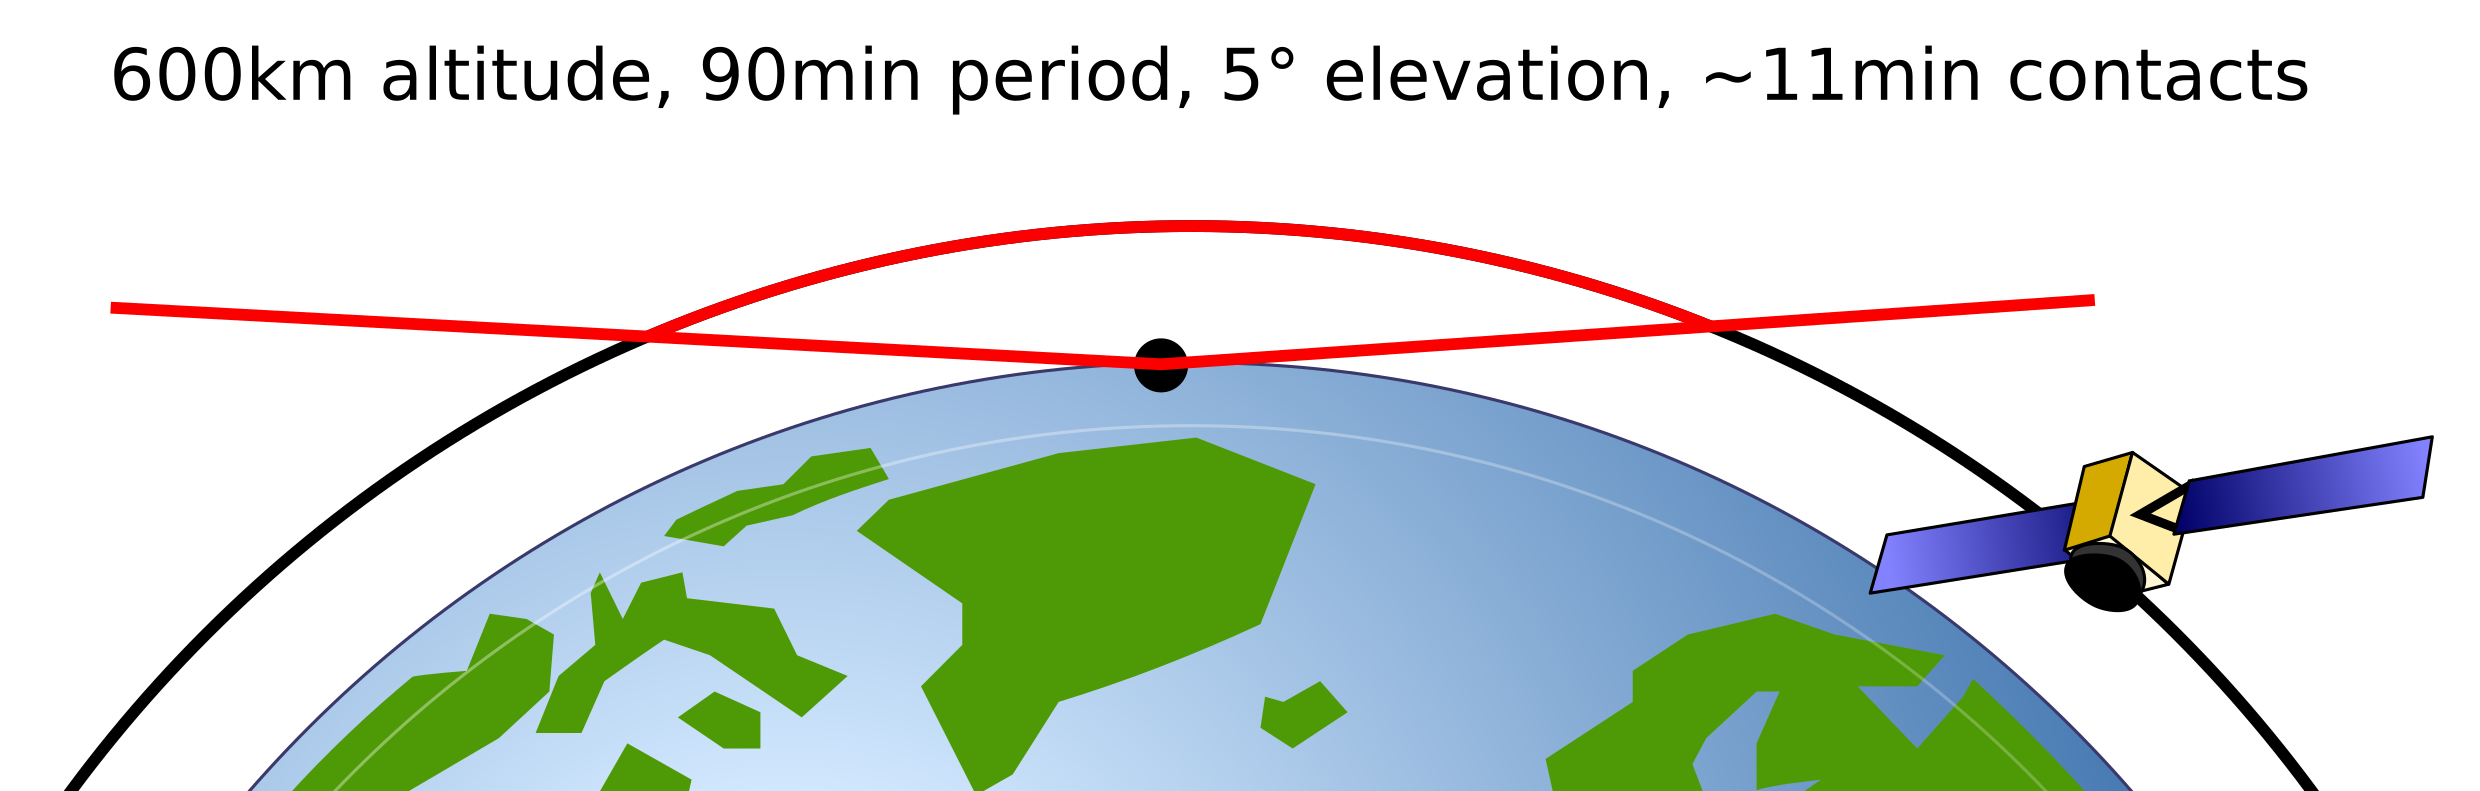
\includegraphics[width=\textwidth]{pass3.png}
  \end{figure}
\end{frame}

\begin{frame}
  \frametitle{Contacts and Passes}
  \begin{figure}[!ht]
    \centering
    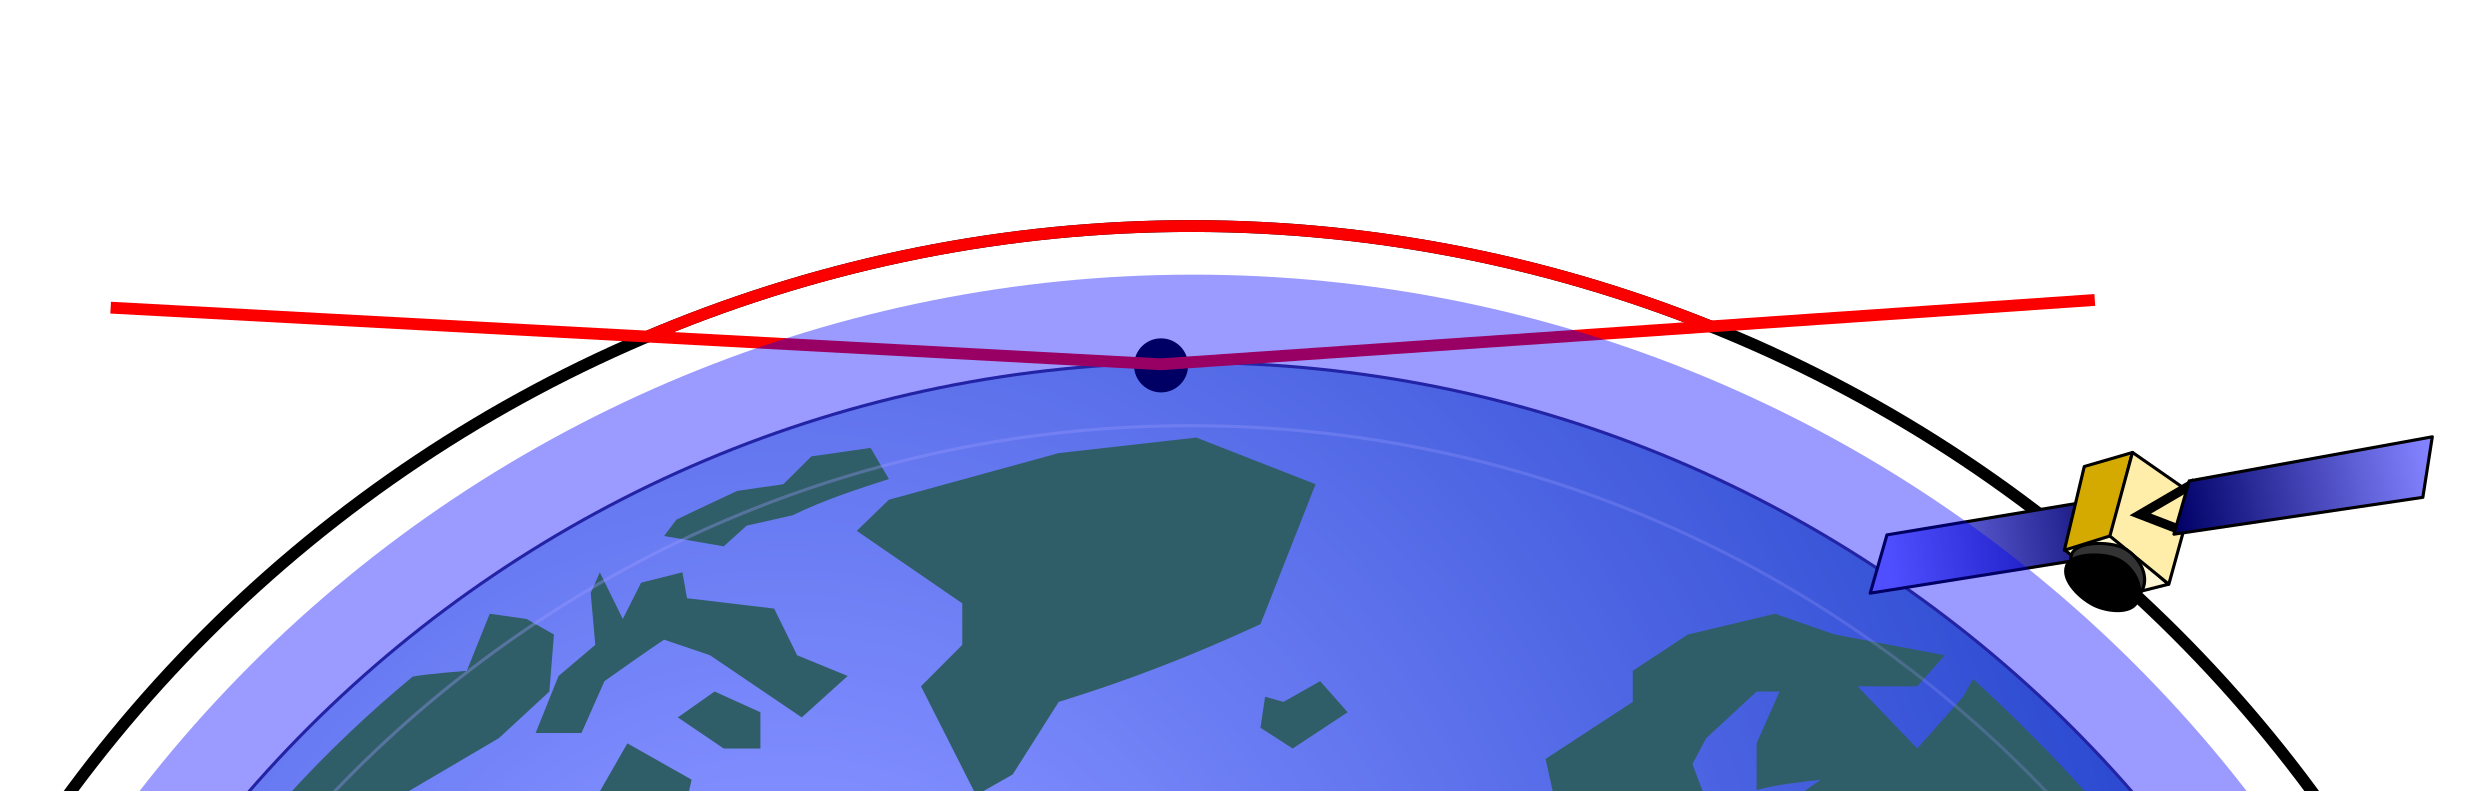
\includegraphics[width=\textwidth]{pass4.png}
  \end{figure}
\end{frame}

\begin{frame}
  \frametitle{Ground Tracks}
  \pause
  \begin{figure}[!ht]
    \centering
    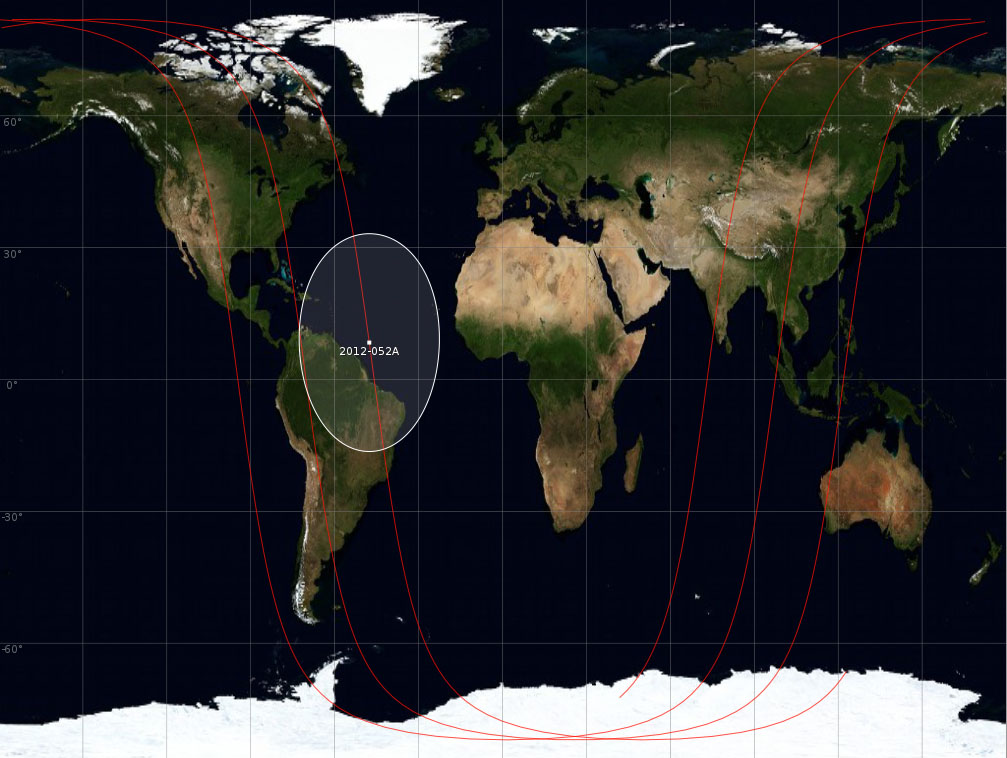
\includegraphics[width=\textwidth]{ground-track.jpg}
  \end{figure}
\end{frame}

\begin{frame}
  \frametitle{Frequency Range}
  \pause
  \begin{figure}[!ht]
    \centering
    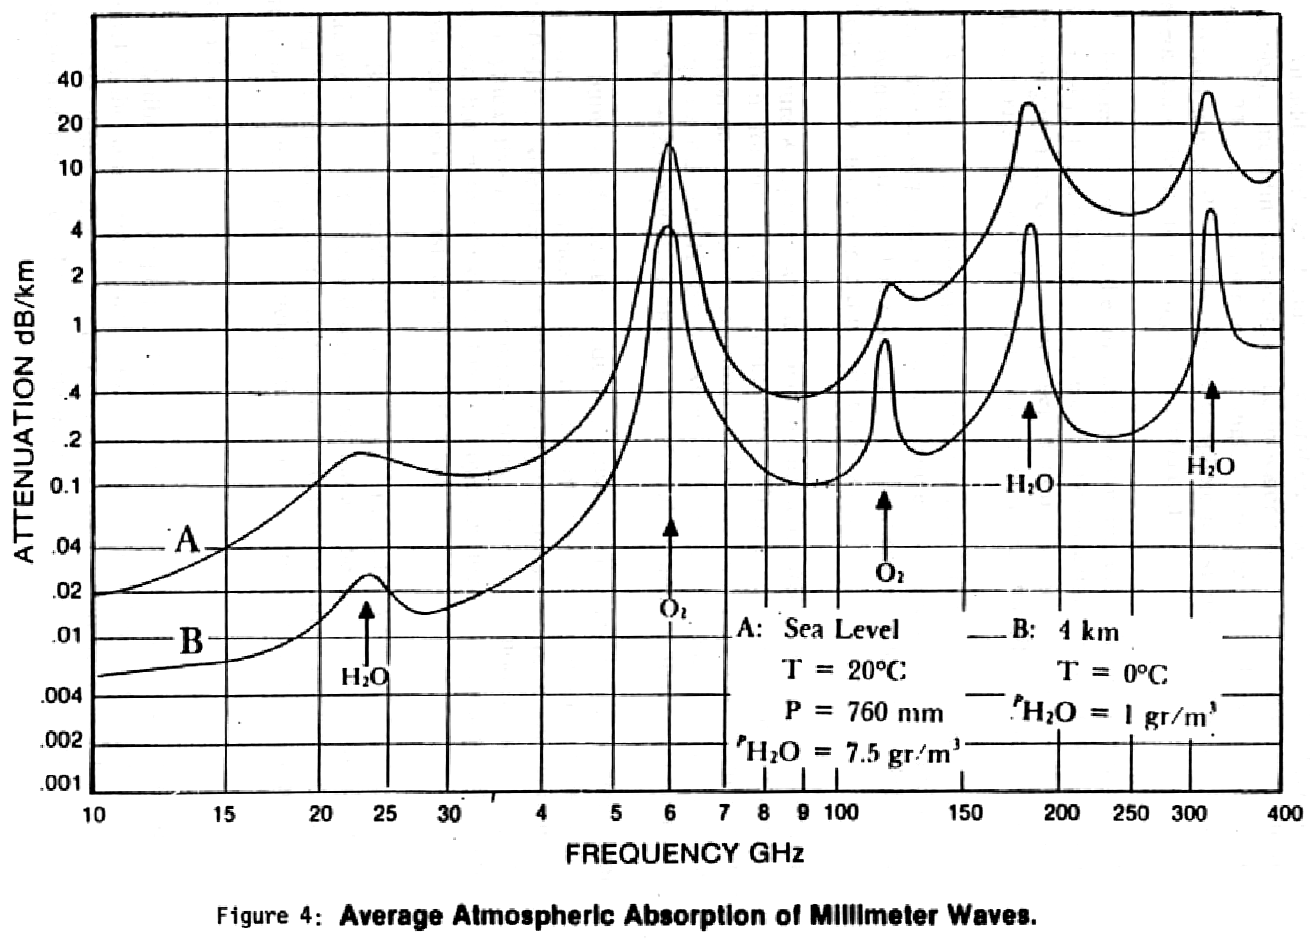
\includegraphics[width=\textwidth]{atmosphere-spectrum.png}
  \end{figure}
\end{frame}

\begin{frame}
  \frametitle{Frequency Range}
  Satellite communication takes place (most commonly) in
  \begin{itemize}
  \item UHF: 430 MHz (CubeSATs) \pause
  \item L-Band: 1-2 Ghz (GNSS, Communications, ADS-B) \pause
  \item S-Band: 2-4 GHz (Telemetry \& Commanding) \pause
  \item X-Band: 8-12 GHz (Payload \& Deep Space) \pause
  \item Ku-Band: 12-18 GHz (TV) \pause
  \item Ka-Band: 26-40 GHz (?)
  \end{itemize}
\end{frame}

\begin{frame}
  \frametitle{Up- and Downlink}
  \pause
  A satellite connection is used for
  \begin{itemize}
  \item downloading satellite telemetry ("house keeping data") \pause
  \item downloading payload data \pause
  \item uploading commands \pause
  \item uploading new software \pause
  \item receiving and sending signals (as a relay)
  \end{itemize}
\end{frame}

\subsection{Phases of Mission Operations}

\begin{frame}
  \frametitle{}
  \vfill
  \begin{center}
    \Large Phases of Mission Operations
  \end{center}
  \vfill
\end{frame}

\begin{frame}
  \frametitle{LEOP}
  \pause
  \textbf{L}aunch and \textbf{E}arly \textbf{O}rbit \textbf{P}hase \pause
  \begin{itemize}
  \item Starts right after separation from transfer vehicle \pause 
  \item Takes 3 days to 4 weeks \pause
  \item 24h per day monitoring and strict agenda \pause
  \item Most important steps: \pause
    \begin{itemize}
    \item First Acquisition \pause
    \item Unfolding of solar panels \pause
    \item Transfer Maneuvers to reach final orbit \pause
    \item First switch-on of star trackers, reaction wheels etc.
    \end{itemize}
  \end{itemize}
\end{frame}

\begin{frame}
  \frametitle{Commissioning or IOT}
  \pause
  \textbf{I}n \textbf{O}rbit \textbf{T}esting \pause
  \begin{itemize}
  \item Follows LEOP \pause
  \item Takes 1 to 6 months \pause
  \item Most important steps: \pause
    \begin{itemize}
    \item Turn-on of payload \pause
    \item Verification of payload \pause
    \item Test of routine operations
    \end{itemize}
  \end{itemize}
\end{frame}

\begin{frame}
  \frametitle{Routine}
  \pause
  \begin{itemize}
  \item Main phase of operations \pause
  \item As much automatic operations as possible \pause
  \item Monitoring of the space craft \pause
  \item Handling of contingencies \pause
  \item Adaptations to changing mission objectives or changing properties of the space craft
  \end{itemize}
\end{frame}

\begin{frame}
  \frametitle{End of Life}
  \pause
  \begin{figure}[!ht]
    \centering
    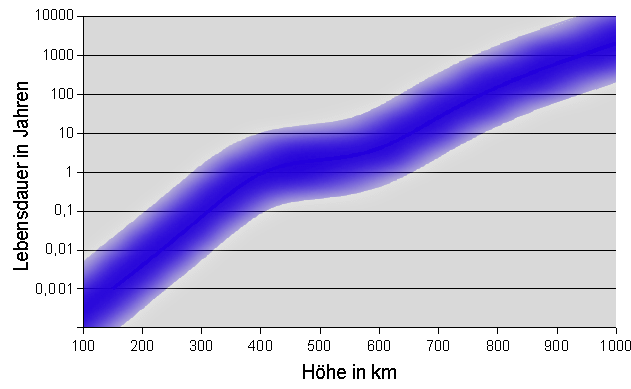
\includegraphics[width=\textwidth]{lifetime.png}
  \end{figure}
\end{frame}

\section{Commanding and Monitoring}

\begin{frame}
  \frametitle{}
  \vfill
  \begin{center}
    \Large Commanding and Monitoring
  \end{center}
  \vfill
\end{frame}

\subsection{TC, TTC and Telemetry}

\begin{frame}
  \frametitle{TCs and TTCs}
  \pause
  \vfill
  Telecommands (TCs) are used to command the S/C \pause
  \vfill
  A TC \pause
  \begin{itemize}
  \item can depend on parameters, \pause
  \item may set values on the S/C, \pause
  \item may switch devices on the S/C or \pause
  \item transport some binary blob \pause
  \end{itemize}
  \vfill
  TCs can be time-tagged $\Longrightarrow$ TTC
  \vfill
\end{frame}

\begin{frame}
  \frametitle{Telemetry}
  \pause
  \vfill
  Telemetry parameters describe the state of the S/C \pause
  \vfill
  They can contain
  \begin{itemize}
  \item binary flags, \pause
  \item numerical data or \pause
  \item binary data \pause
  \end{itemize}
  \vfill
  Should consume as less bandwidth as possible! \pause
  \vfill
  A S/C can easily have 20000 such parameters \pause
  \vfill
  After processing this is saved in a space craft database
\end{frame}

\begin{frame}
  \frametitle{Examples for TTCs during a maneuver}
  \pause
  \centering
  \begin{tabular}{|c|c|}\hline
    Time & Action \\ \hline
    $t_0-00:60:00$ & Check preconditions \\
    $t_0-00:59:52$ & Heat thrusters \\
    $t_0-00:11:00$ & Switch on additional telemetry \\
    $t_0-00:09:40$ & Turn off safeguards \\
    $t_0-00:06:40$ & Rotating space craft \\
    $t_0$ & Burn starts \\
    $t_0+1.1\cdot \text{burn time}$ & Additional safeguard STOP command \\
    $t_0+00:00:01$ & Rotate back \\
    $t_0+00:13:00$ & Turn off heaters \\
    $t_0+00:14:54$ & Turn back to old mode \\ \hline
  \end{tabular}
\end{frame}

\subsection{Flight and Ground Procedures}

\begin{frame}
  \frametitle{Flight Procedures}
  \pause
  A flight procedure (FOP) is a sequence of \pause
  \begin{itemize}
  \item TM-checks, \pause
  \item TCs and \pause
  \item some simple logics such as loops or conditions
  \end{itemize}
  \vfill
  Does a specific task on the S/C in a consistent and safe manner
  \vfill
  Preparation and Validation of FOPs is one of the main works in preparation phase for the mission
\end{frame}

\begin{frame}
  \frametitle{Ground Procedures}
  \pause
  Similarly to FOPs, fround procedures (GOPs) are explicit sequences how to do a specific task in the ground segment \pause
  \vfill
  Needs to be simple, concise and doable at 3am by anybody in the OPS team
  \vfill
  Examples: \pause
  \begin{itemize}
  \item How to restart some software \pause
  \item How to command a change of the mode of a S/C via a FOP
  \end{itemize}
\end{frame}

\section{Subsystems}

\begin{frame}
  \frametitle{}
  \vfill
  \begin{center}
    \Large Subsystems
  \end{center}
  \vfill
\end{frame}

\begin{frame}
  \frametitle{Control Room}
  \pause
  \begin{figure}[!ht]
    \centering
    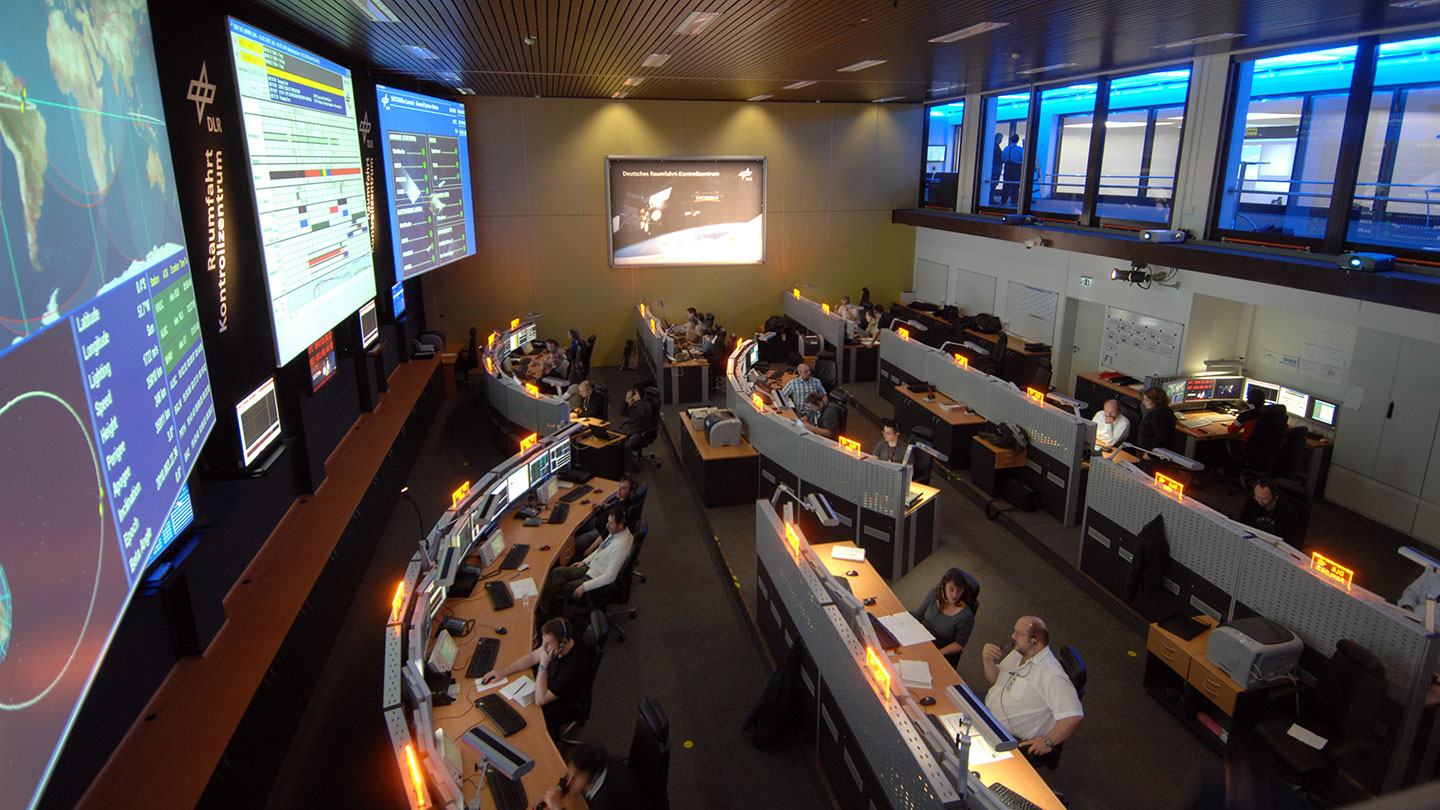
\includegraphics[width=\textwidth]{k1.jpg}
  \end{figure}
\end{frame}

\begin{frame}
  \frametitle{FDS and AOCS}
  \pause
  Flight Dynamics (FDS) does \emph{orbit propagation},\pause \emph{ground station visibilities}\pause and \emph{maneuver calculations}
  \vfill
  Attitude and Orbital Control System (AOCS) is responsible for S/C operations regarding \emph{attitude},\pause \emph{tumbling},\pause \emph{maneuver execution}\pause and \emph{positioning}
\end{frame}

\begin{frame}
  \frametitle{Target-Pointing-Mode}
  \pause
  \begin{figure}[!ht]
    \centering
    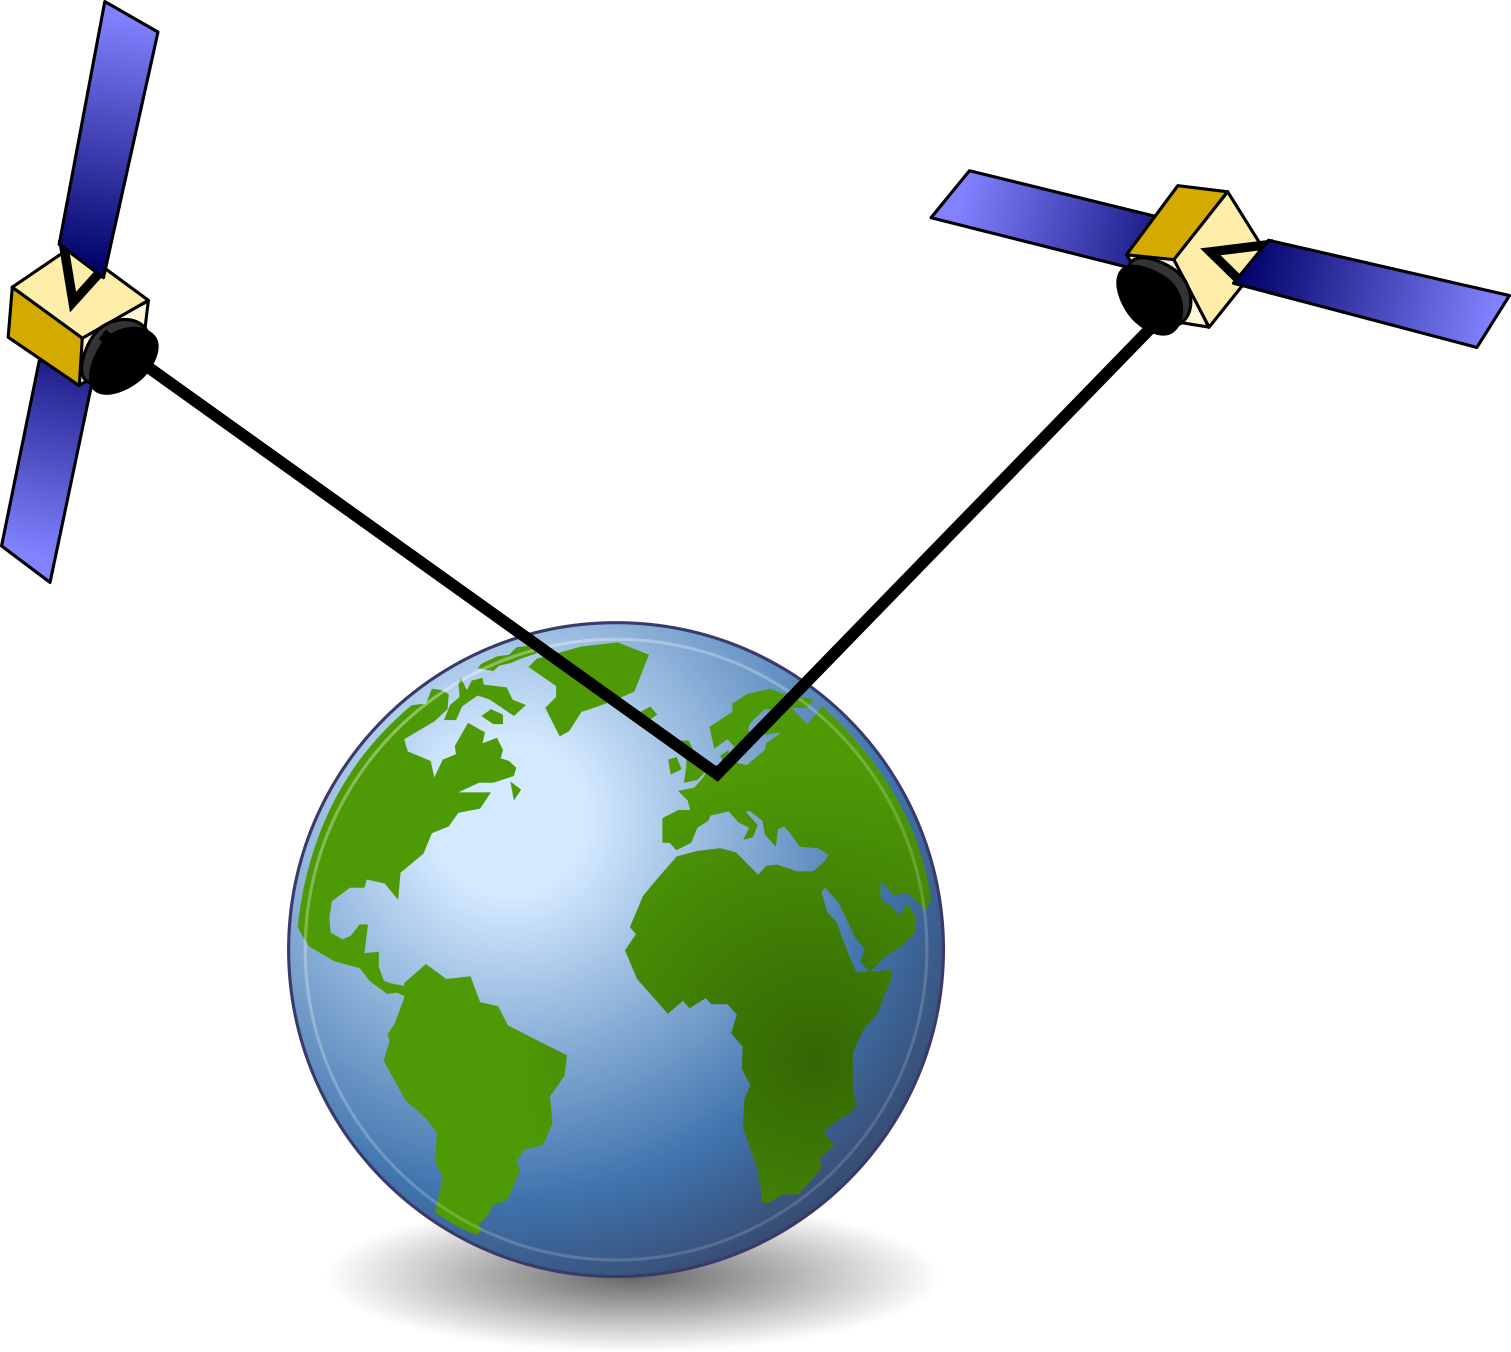
\includegraphics[width=0.8\textwidth]{target-pointing-mode.png}
  \end{figure}
\end{frame}

\begin{frame}
  \frametitle{Sun-Pointing-Mode}
  \begin{figure}[!ht]
    \centering
    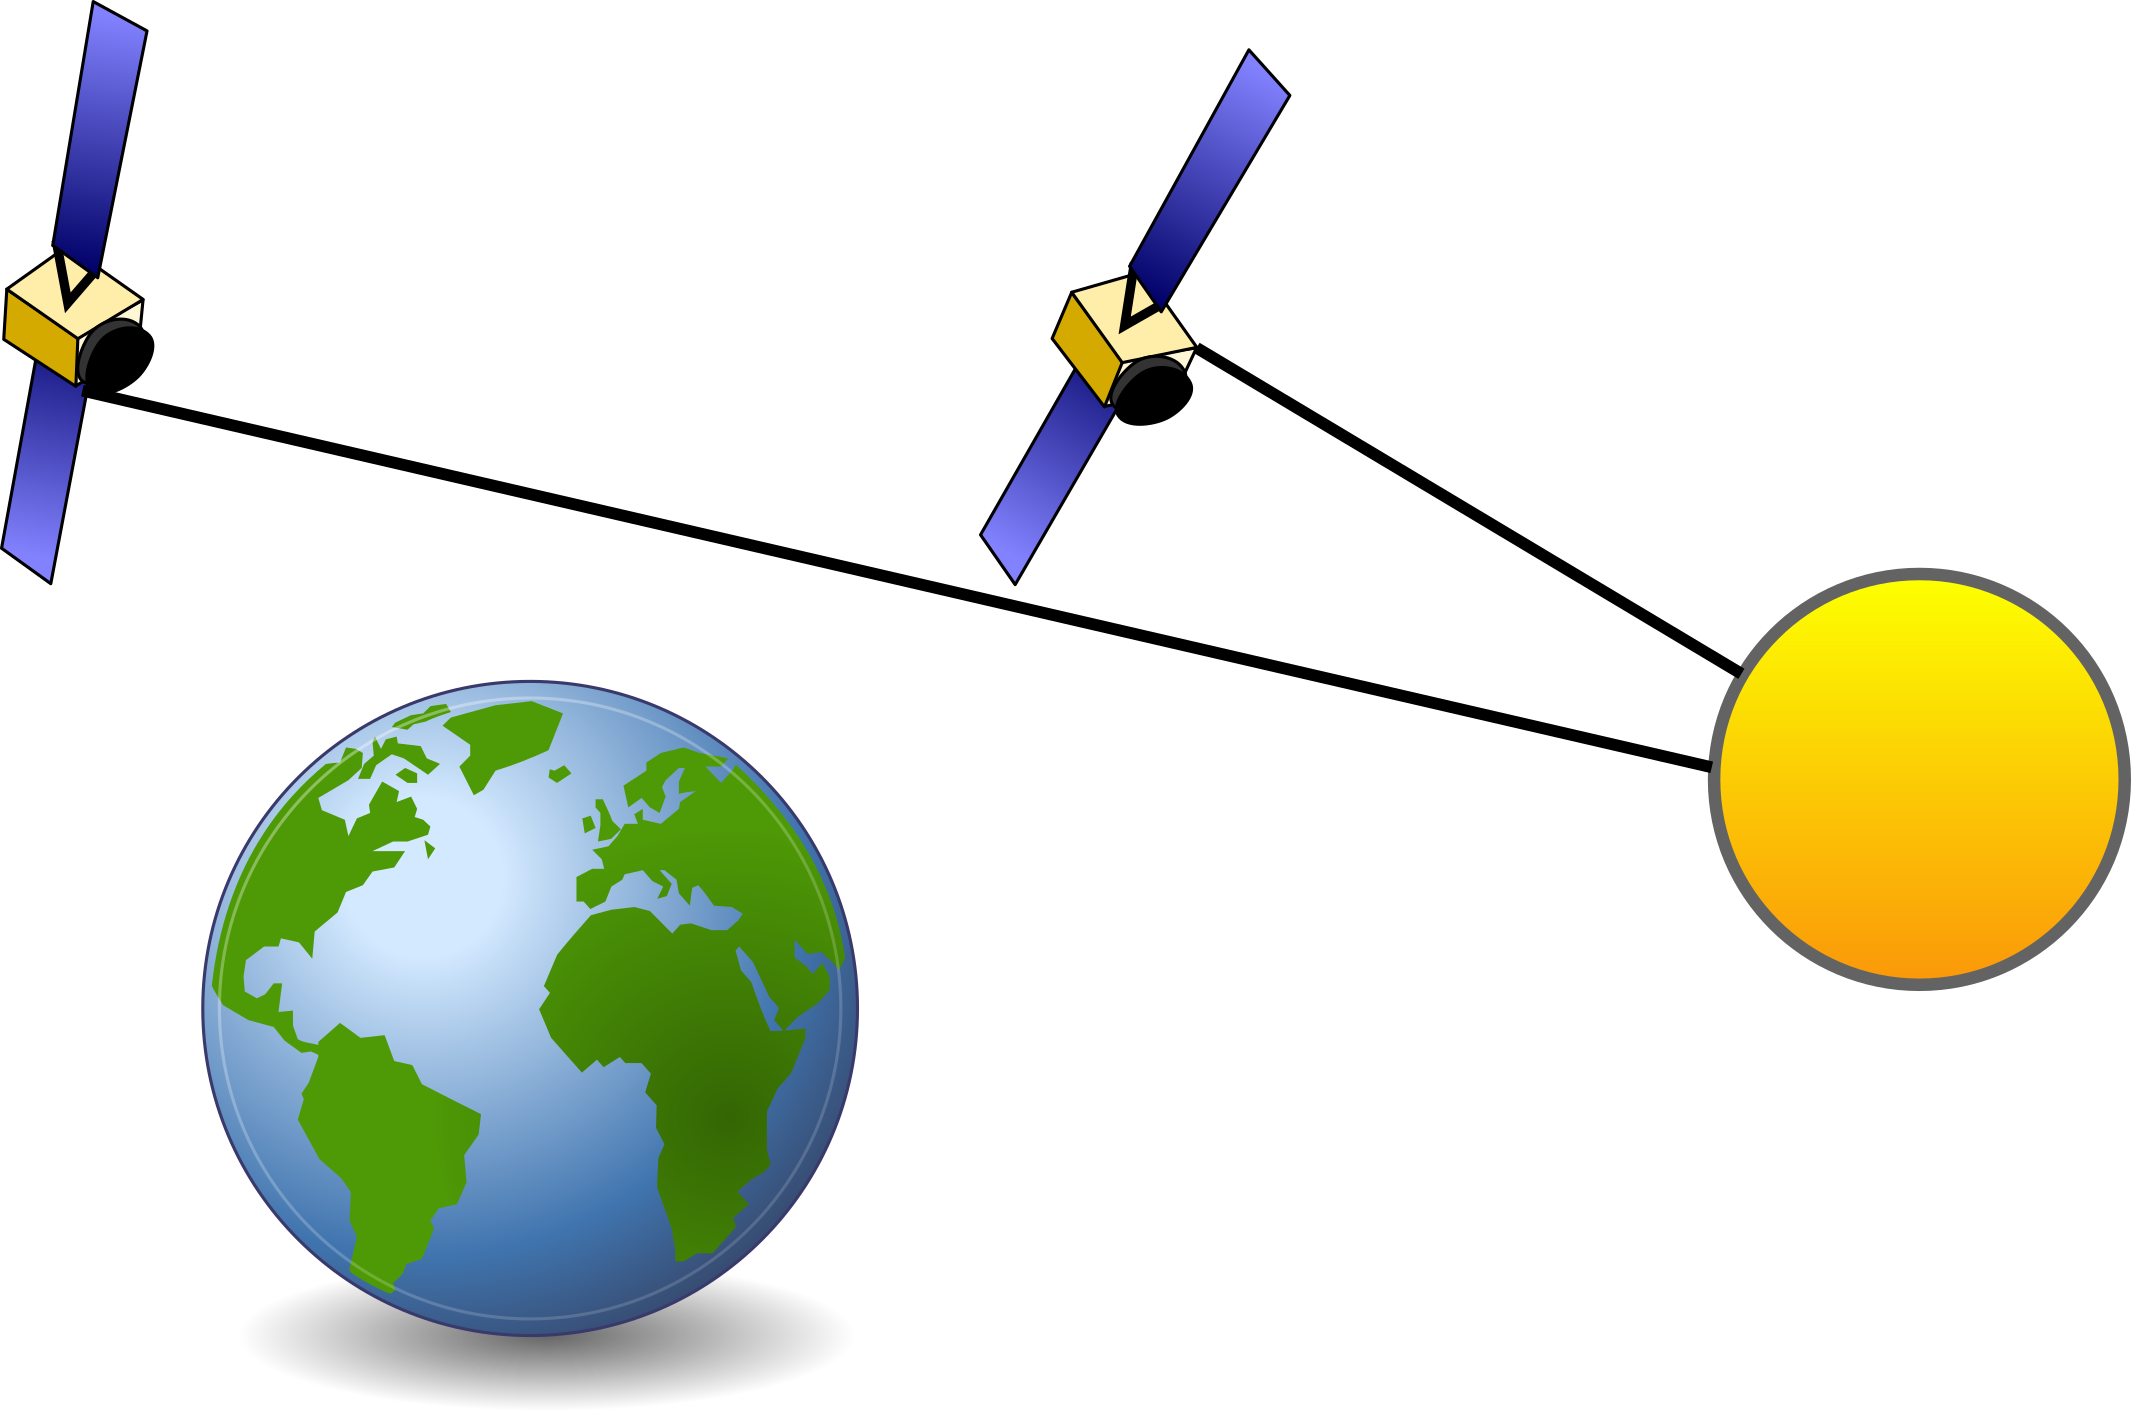
\includegraphics[width=\textwidth]{sun-pointing-mode.png}
  \end{figure}
\end{frame}

\begin{frame}
  \frametitle{Data and TM/TC}
  \pause
  Data and TM/TC are responsible for
  \begin{itemize}
  \item Acquisition and maintenance of signal/TM-flow, \pause
  \item Ranging, \pause
  \item Data processing    
  \end{itemize}
\end{frame}

\begin{frame}
  \frametitle{SCOS}
  \begin{figure}[!ht]
    \centering
    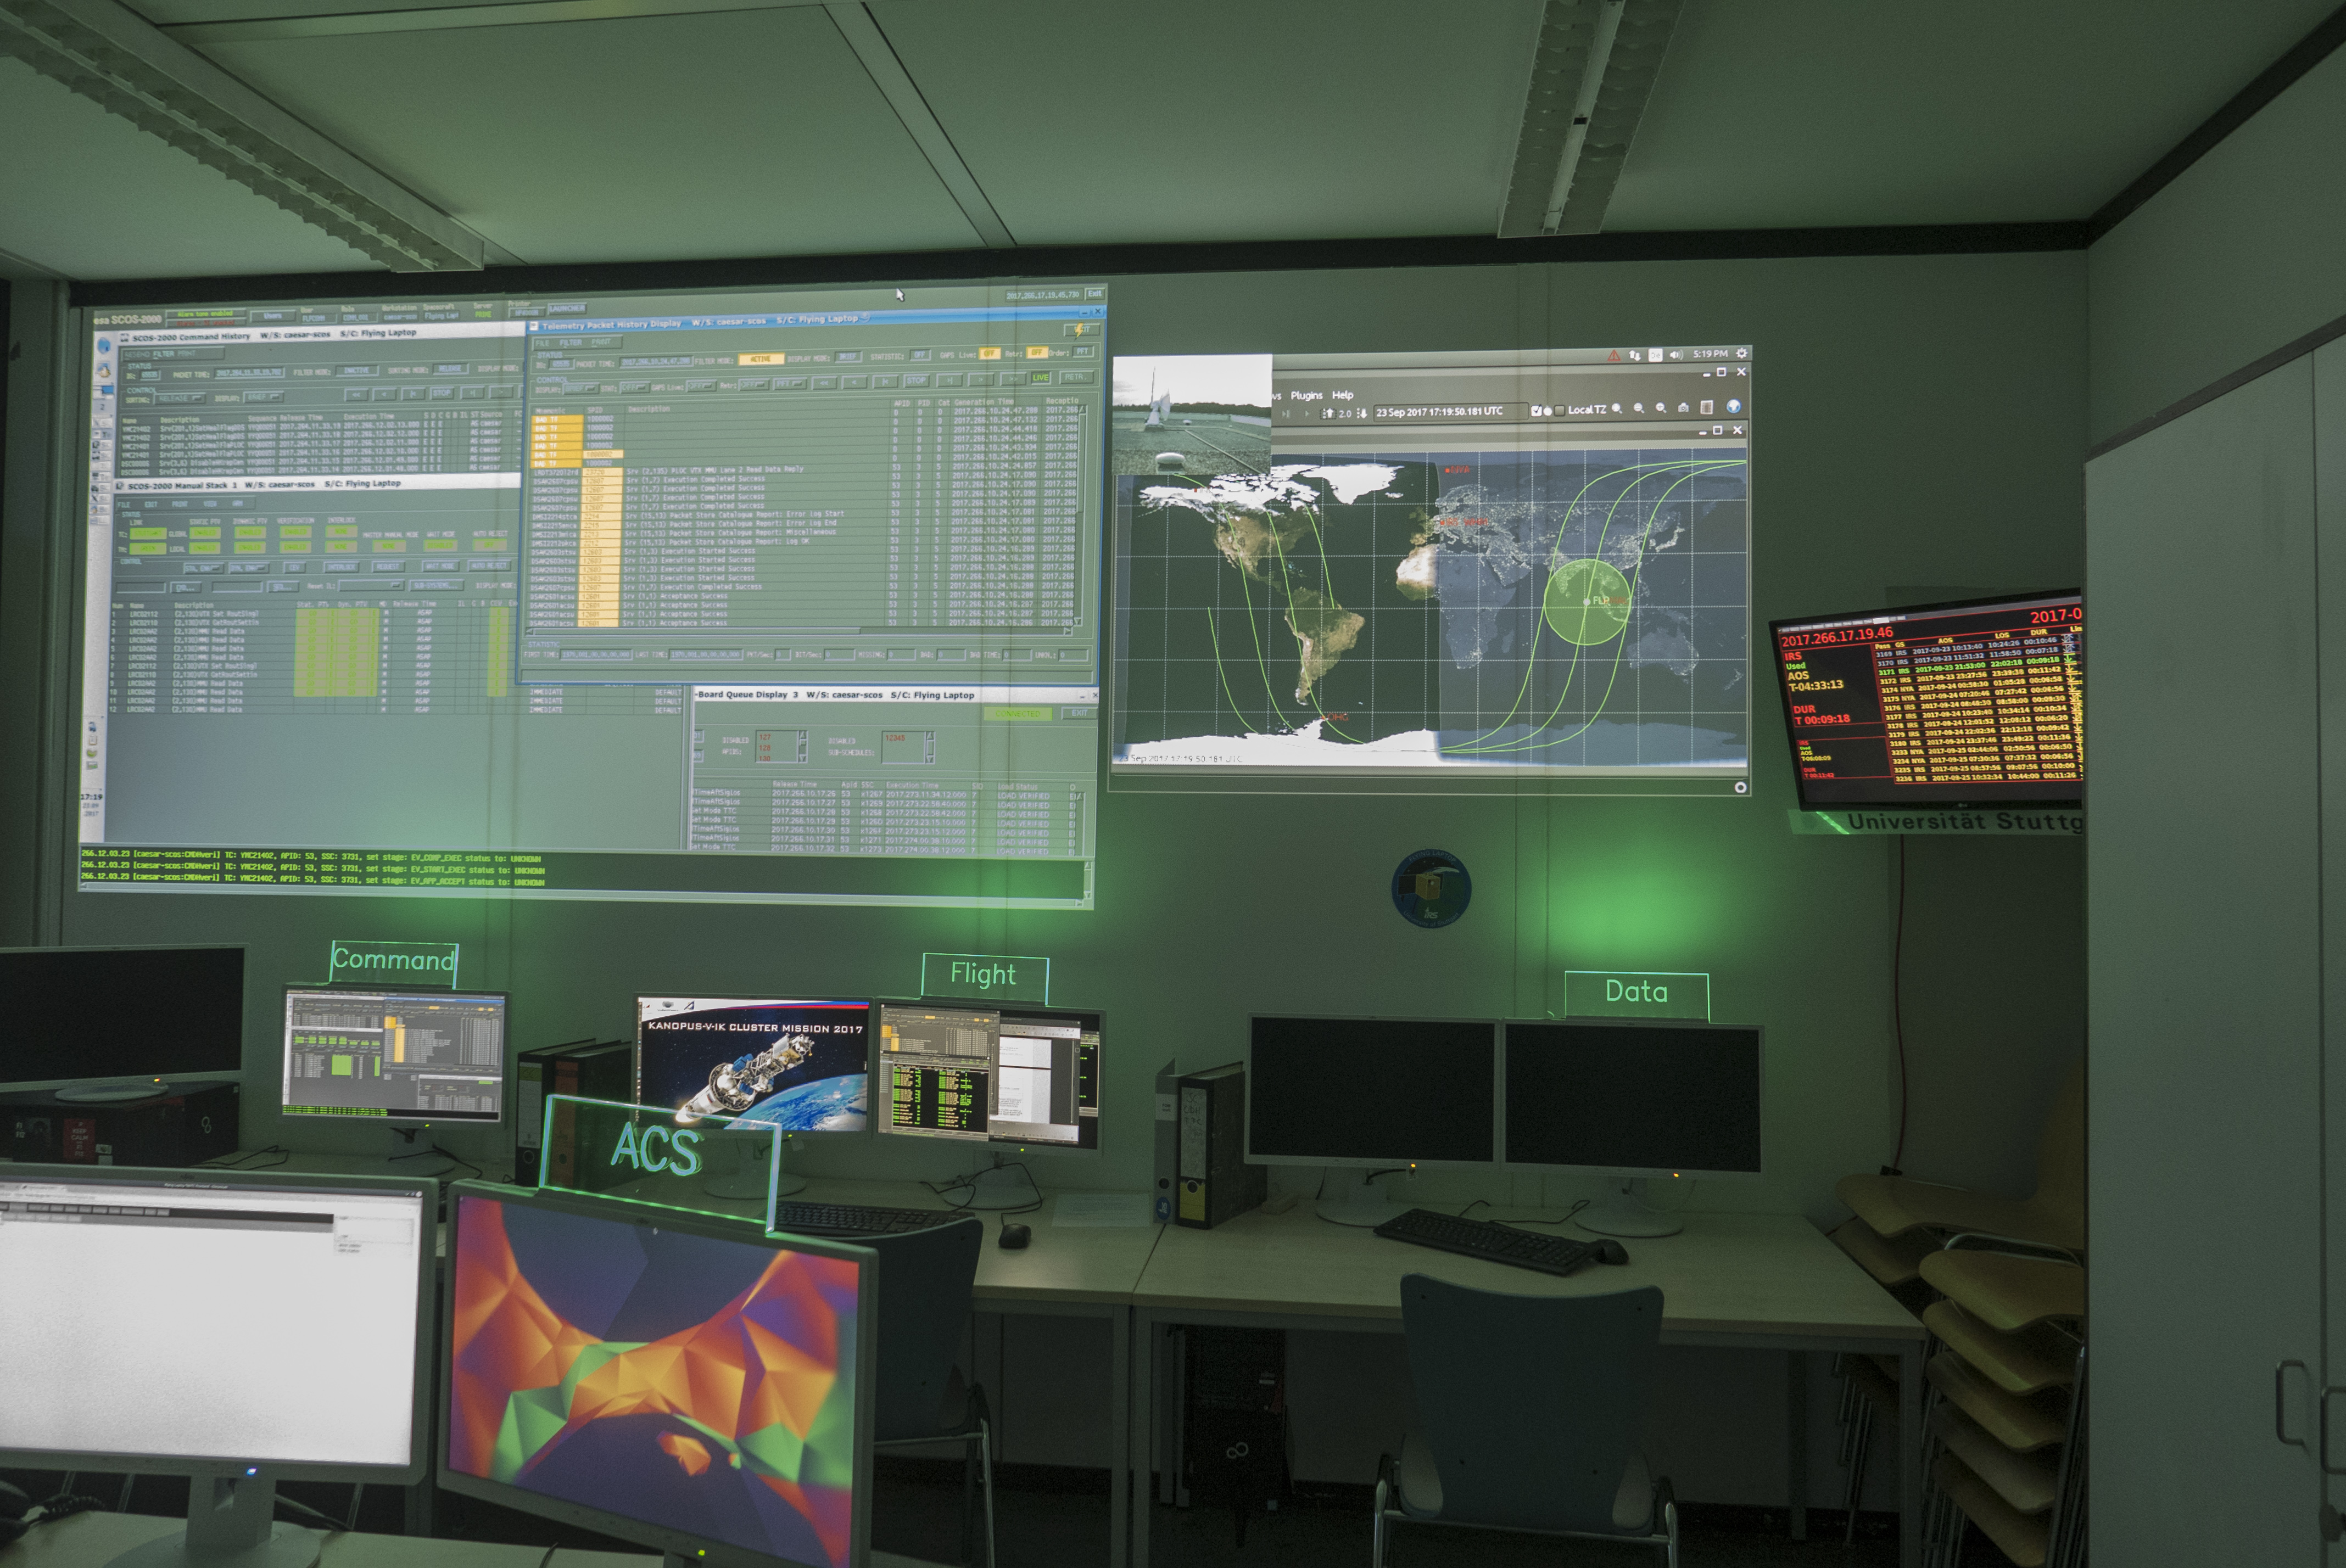
\includegraphics[width=0.8\textwidth]{scos.jpg}
  \end{figure}
\end{frame}

\begin{frame}
  \frametitle{PTR}
  \pause
  Power and Thermal (PTR) monitor
  \begin{itemize}
  \item battery state and \pause
  \item temperatures on the S/C
  \end{itemize}
  \vfill
  Temperatures can easily range from $-60\deg C$ to $+100\deg C$
  \vfill
  Long term monitoring very important
\end{frame}

\begin{frame}
  \frametitle{MiPL}
  \pause
  Mission Planning (MiPL) takes care of
  \begin{itemize}
  \item planning S/C activities in a consistent and conflict-free manner, \pause
  \item executing automated FOPs in routine operations and \pause
  \item detailed planning during the LEOP
  \end{itemize}
\end{frame}

\begin{frame}
  \frametitle{Sequence of Events}
  \pause
  TODO add picture sample SoE
\end{frame}

\section{Contingencies}

\begin{frame}
  \frametitle{}
  \vfill
  \begin{center}
    \Large Contingencies
  \end{center}
  \vfill
\end{frame}

\begin{frame}
  \frametitle{Flight and Engineering Model}
  \pause
  There exists an engineering model of the S/C and simulators for \pause
  \begin{itemize}
  \item validation of FOPs, \pause
  \item training of operators during preparation before launch, \pause
  \item connection tests and \pause
  \item reproducing errors on the flight model
  \end{itemize}
\end{frame}

\begin{frame}
  \frametitle{Procedure in Case of Contingency}
  \pause
  \vfill
  Stay calm! \pause
  \vfill
  Verify your input data \pause
  \vfill
  Call people responsible for that sub system \pause
  \vfill
  Analyze possible failure causes ("Next pass ...") \pause
  \vfill
  Test solution \pause
  \vfill
  Execute solution
\end{frame}

\begin{frame}
  \frametitle{Example Contingency: TV-SAT 1}
  \pause
  \vfill
  German-French TV satellite from 1987 \pause
  \vfill
  First acquisition successful, but solar-array deployment switch said that solar panels were only partially deployed \pause
  Some immediate actions:
  \begin{itemize}
  \item Check ground database for flip inversion \pause
  \item Check output power of affected solar array \pause
  \item Manual deployment command was sent \pause
  \item Redundant deployment pyros were fired \pause
  \end{itemize}
  \vfill
  $\Longrightarrow$ We have a problem!
\end{frame}

\begin{frame}
  \frametitle{Example Contingency: TV-SAT 1}
  \pause
  \vfill
  Offline analysis by the satellite manufacturer showed more than $50$ possible failure cases $\Longrightarrow$ We need tests! \pause
  \vfill
  \begin{figure}[!ht]
    \centering
    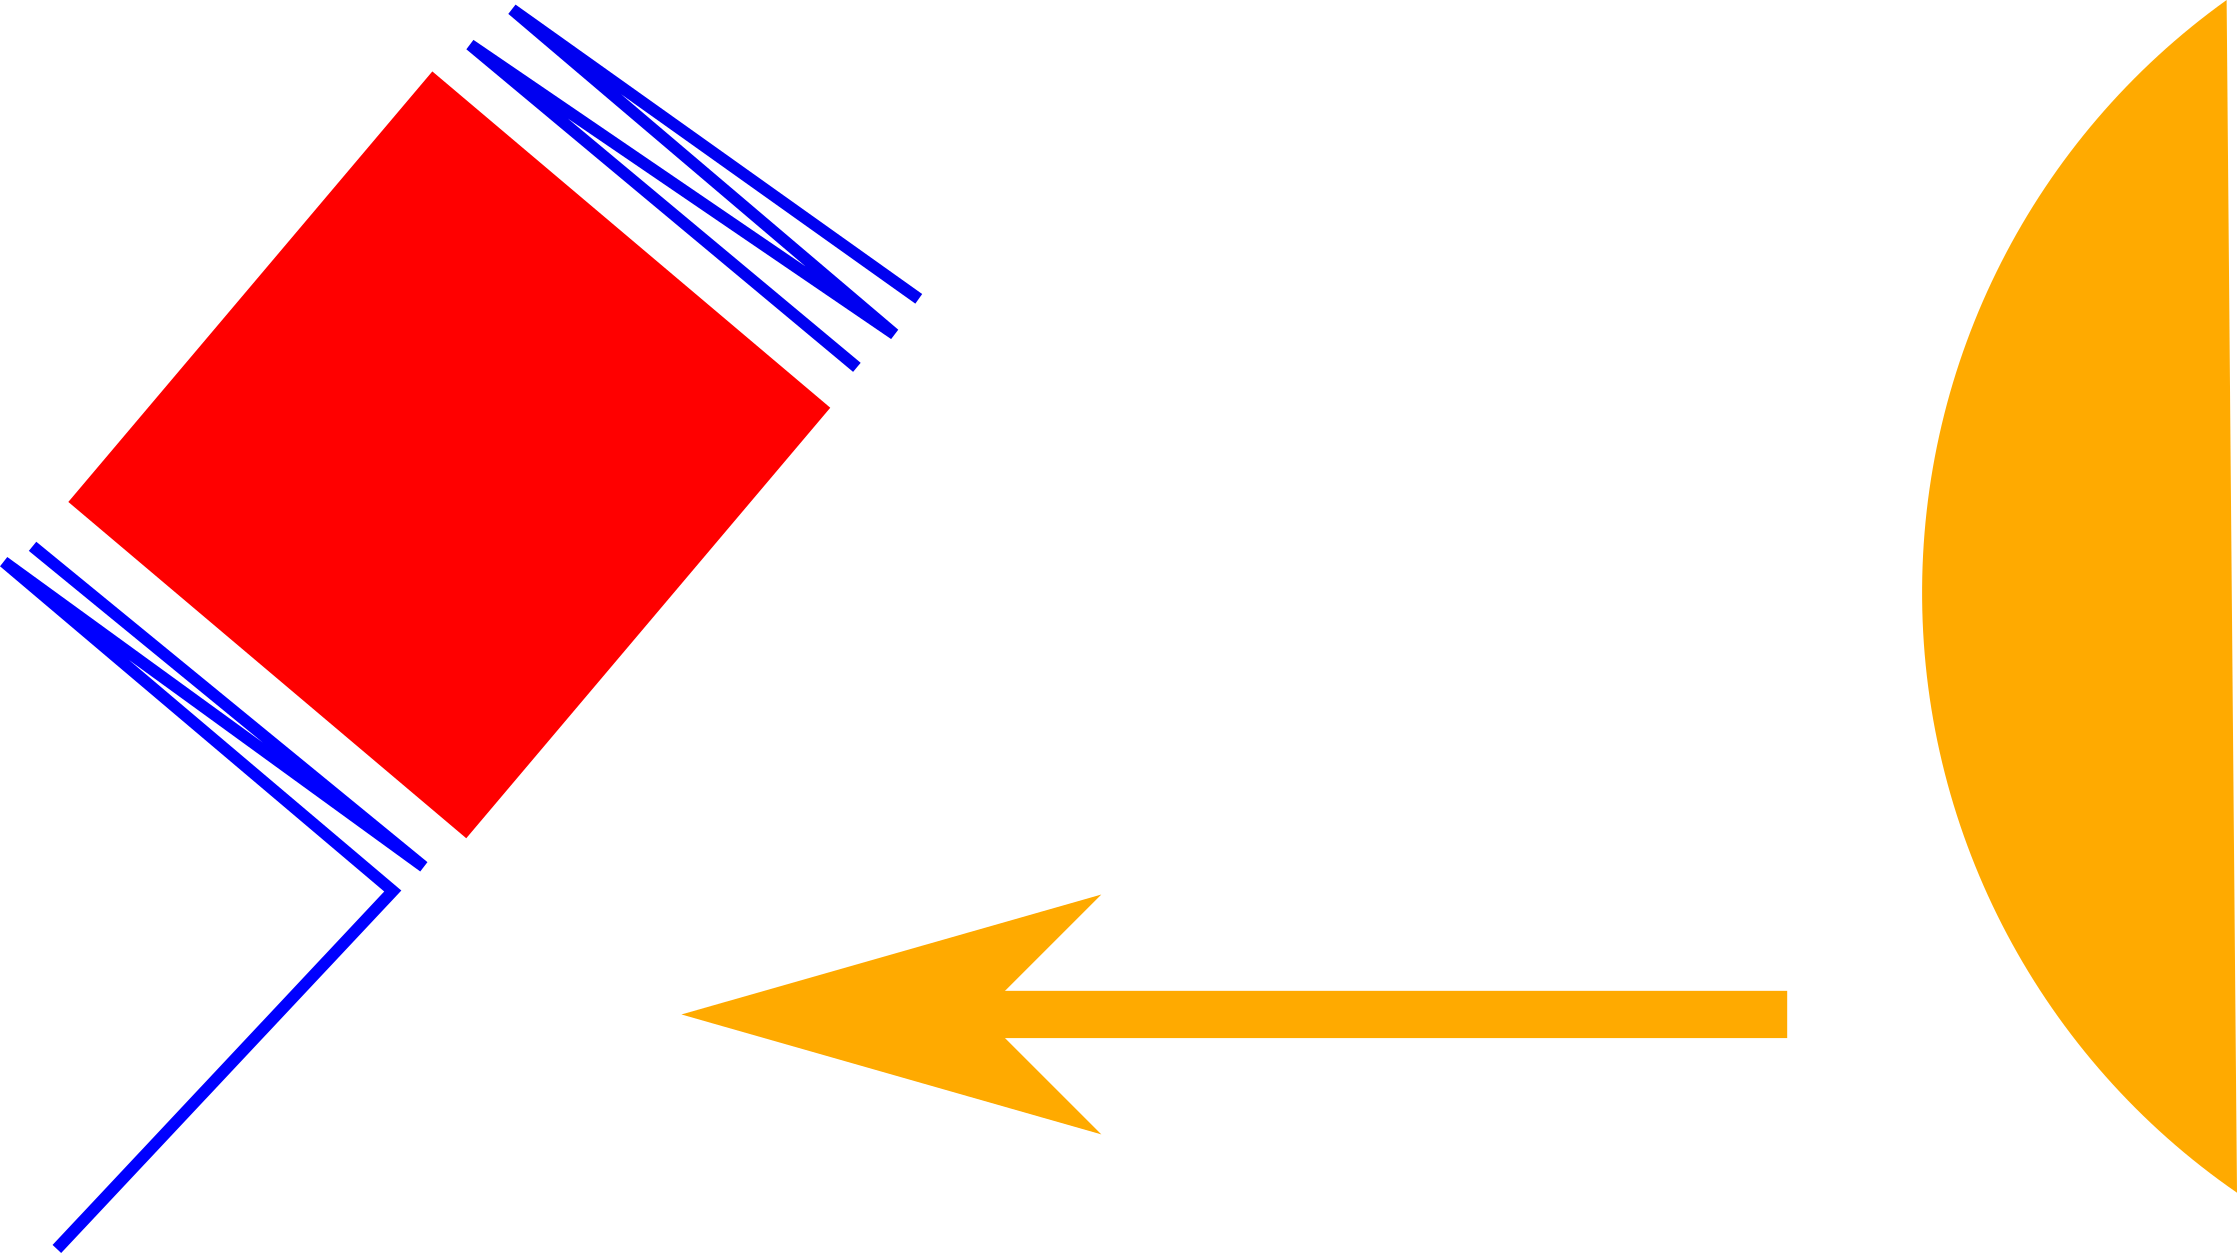
\includegraphics[width=0.6\textwidth]{tvsat1.png}
  \end{figure}
\end{frame}

\begin{frame}
  \frametitle{Example Contingency: TV-SAT 1}
  \begin{figure}[!ht]
    \centering
    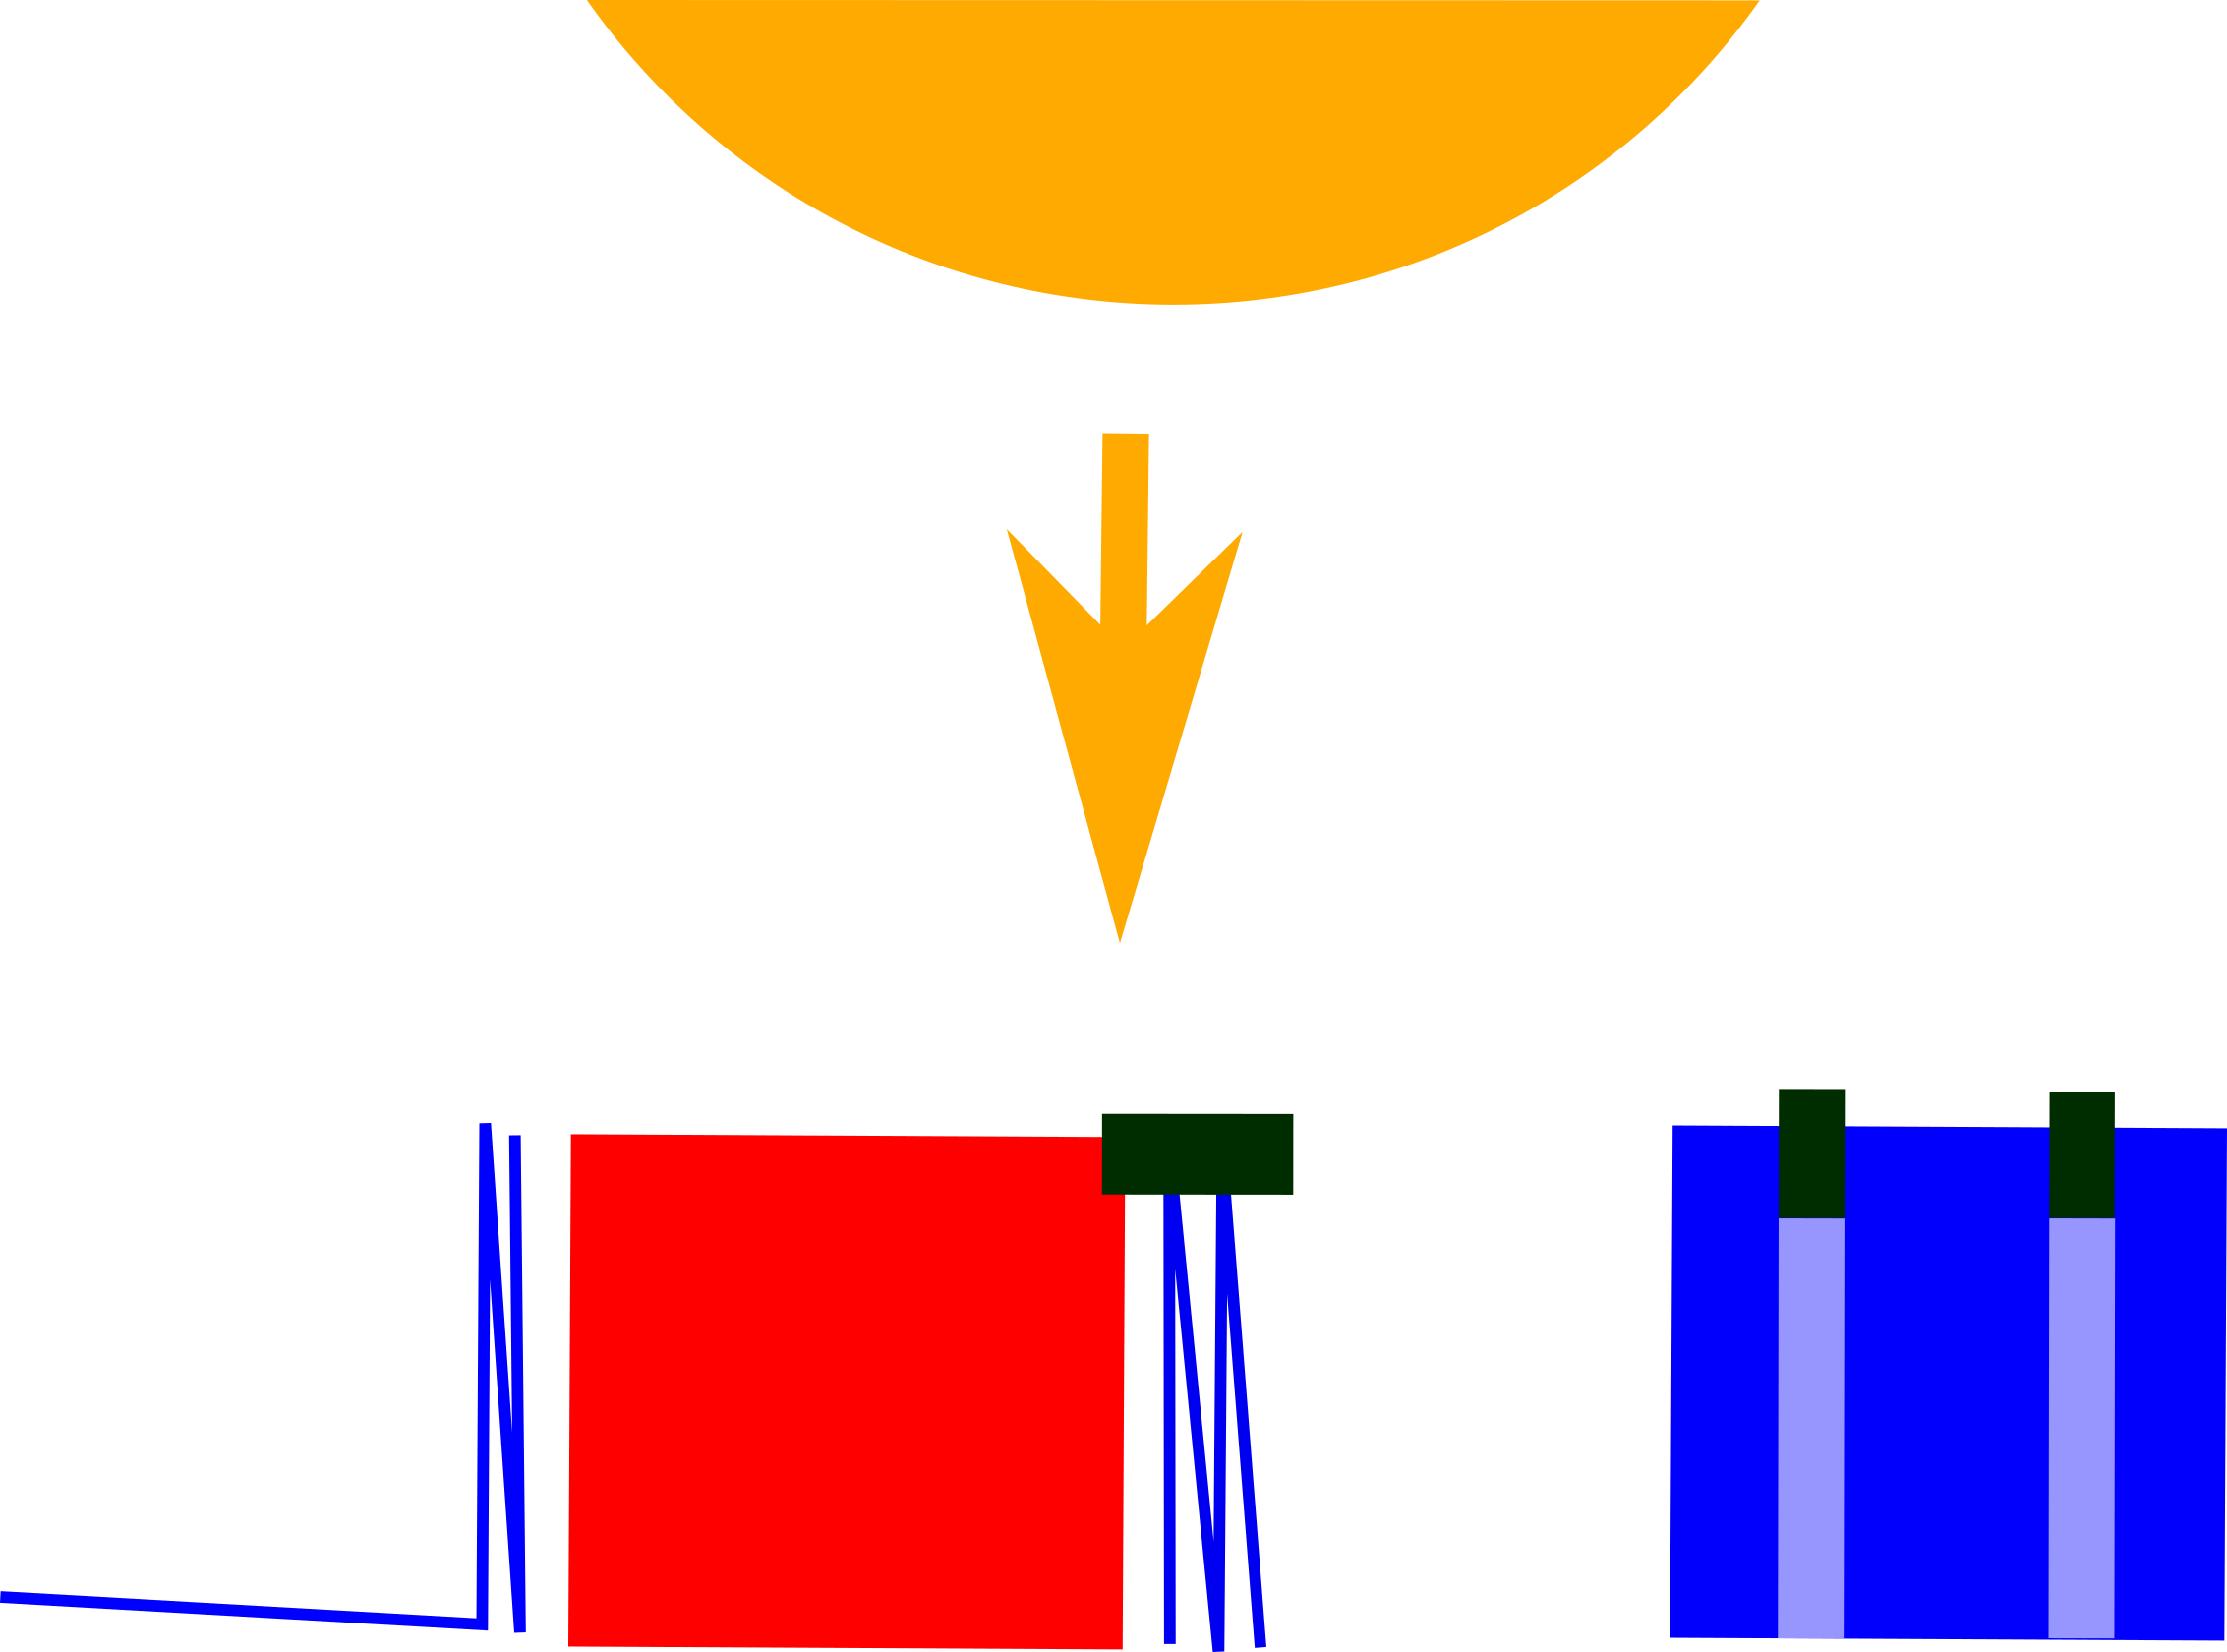
\includegraphics[width=0.6\textwidth]{tvsat2.png}
  \end{figure}
  \pause
  More tests (Rotating S/C in another axis and measureing flux, shaking of S/C to find resonance frequencies) all showed: \pause
  The solar panels were indeed not deployed.
\end{frame}

\begin{frame}
  \frametitle{Example Contingency: TV-SAT 1}
  Recovery attempts: \pause
  \begin{itemize}
  \item Fast rotation (~1g centrifugal force) to loosen stirrups \pause
  \item Performing pulsed boosts to excite resonance frequencies \pause
  \item Heating and cooling panel and stirrups \pause
  \item Antenna deployment causes a shock to the S/C  \pause
  \end{itemize}
  \vfill
  All in all: no success :-( \pause
  
  But usually everything works fine!
\end{frame}

\begin{frame}
  \frametitle{Questions?}
  \vfill
  \begin{center}
    \Large Thank you and enjoy the rest of the congress!
  \end{center}
  \vfill
\end{frame}


\end{document}
